\documentclass[a4paper,11pt]{article}
\usepackage[utf8]{inputenc}
\usepackage{graphicx}
\usepackage{gensymb}
\usepackage{amsmath}

\setlength{\textwidth}{475pt}
\setlength{\textheight}{660pt}
\setlength{\hoffset}{-22mm}
\setlength{\voffset}{-25mm}

\setcounter{secnumdepth}{5}
\setcounter{tocdepth}{5}

%opening
\title{The design and construction of the MICE Electron-Muon Ranger}
\author{}

\begin{document}

\maketitle

\begin{abstract}
The Electron-Muon Ranger (EMR) is a totally active scintillator detector installed in the beam of the Muon Ionization
Cooling Experiment (MICE) \cite{MICEweb}. The experiment will demonstrate ionization cooling, an essential technology needed
for the realization of a Neutrino Factory and/or Muon Collider. The EMR is aimed at measuring the properties of the low
energy beam composed of muons, electrons and pions, performing the identification particle by particle. The detector is
made of 48 stacked layers alternately measuring $X$ and $Y$ coordinates. Each layer consists of 59 triangular scintillator
bars. The read-out is based on FPGA custom made electronics and commercially available modules. This article will describe
the construction of the detector, starting with the design of the detector up to its final commissioning with particle beam.
\end{abstract}

\section{Introduction}
\subsection{Ionization cooling}
The Neutrino Factory based on a high-energy muon storage-ring is the ultimate tool to study the neutrino mixing matrix
and is established as the best facility to discover, and study the possible leptonic CP violation. It will produce the
most intense, pure and focused neutrino beam ever achieved and is also the first step towards a $\mu^+ \mu^-$ collider.
The Neutrino Factory accelerator complex will use as a sources muons, produced as a tertiary beam. A proton beam bombarding
a target will produce pions. These pions will be captured and focused in a high-field solenoid channel and will decay
to muons, creating a low energy muon beam with very large emittance.  The emittance of the muons needs to be reduced,
i.e the muon must be “cooled”, so that the beam can be accelerated efficiently.

\begin{figure}[htb]
 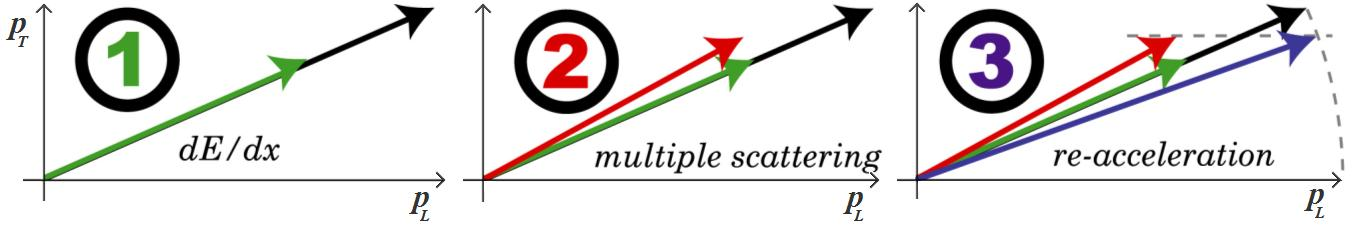
\includegraphics[width=1.\linewidth]{./ICool.png}
 \caption{Ionization cooling principle: \ \ 1. Energy loss by ionization ($dE/dx$ reduces $P_L$ and $P_T$)
    2. Heating from multiple scattering
    3. $P_L$ restored by RF cavities    
   }
 \label{icool}     
\end{figure}

Ionization cooling \cite{icool1} (Fig.\ \ref{icool}) provides the only practical solution to this problem,
because it is fast enough to cool the beam within the muon lifetime ($\tau_\mu \sim 2.2 \ \mu s$). The cooling effect is
accomplished by passing the muons through a low-Z material (\textquotedblleft absorber\textquotedblright), in which they
loses energy via ionization, reducing both the longitudinal and the transverse components of the momentum. Later the
longitudinal momentum is restored by accelerating cavities. The net effect is a reduction of the beam emittance. To
maximize cooling we need the absorber to be placed at a position where the transverse momentum $P_T$ has a maximum
(the transverse betatron function $\beta_{\perp}$ has a minimum).

\subsection{MICE}
The international Muon Ionization Cooling Experiment (MICE) \cite{MICEweb} is under development at the Rutherford Appleton
Laboratory (UK). The goal of the experiment is to build a section of a cooling channel that can demonstrate the principle
of Ionization cooling and to verify its performance in a muon beam. 

Since energy loss by ionization and multiple Coulomb scattering are momentum dependent, the ionization cooling effect is
momentum dependent. MICE (Fig. \ref{mice}) uses variety of muon beams of limited intensity, having central momenta in the
range $140 - 240 \ MeV/c$ and a momentum spread of $\sim 20 \ MeV/c$. These muon beams are generated using a titanium target
\cite{target} which is dipped into the ISIS proton beam \cite{isis}. Produced secondary and tertiary particles are captured,
momentum-selected and transported to the cooling section by a system of magnets which includes: $5\ T$ superconducting pion
decay solenoid, two dipole magnets, nine quadrupole magnets and a mechanism for inflation of the initial emittance called Diffuser.

The cooling section of MICE, is similar to the cooling channel for the International Design Study
for the Neutrino Factory \cite{ids-nf}. It consists of one primary lithium-hydride (LiH) absorber, two secondary absorbers,
two focus coils and two 201 MHz RF cavities. The two superconducting focus-coil modules provide strong focusing at the
absorber, ensuring that the transverse betatron function is minimised at this position and enhancing the cooling effect. 
All beam particles are detected individually by two identical Scintillating fiber trackers in 4T
solenoids, situated upstream and downstream of the cooling section. The beam emittance is reconstructed, by measuring the
spatial coordinates and momentum ($x,y,p_x,p_y,p_z$) of each muon.

The particle content of the beam is measured by a dedicated system of detectors situated upstream and downstream of the
cooling section and designed to provide precise muon, pion and electron identification. The upstream part includes two
Time-of-flight hodoscopes (TOF0 and TOF1) and a Cherenkov detectors (Ckov). The downstream part combines another 
Time-of-flight hodoscope (TOF2) and a calorimeter system. The calorimeter system consists of the KLOE-Light (KL)
lead-scintillator sampling calorimeter, similar to the KLOE design [30], but with thinner lead foils, serving
as a preshower for the totally-active Electron-Muon ranger (EMR), situated behind him.

\begin{figure}[h]
 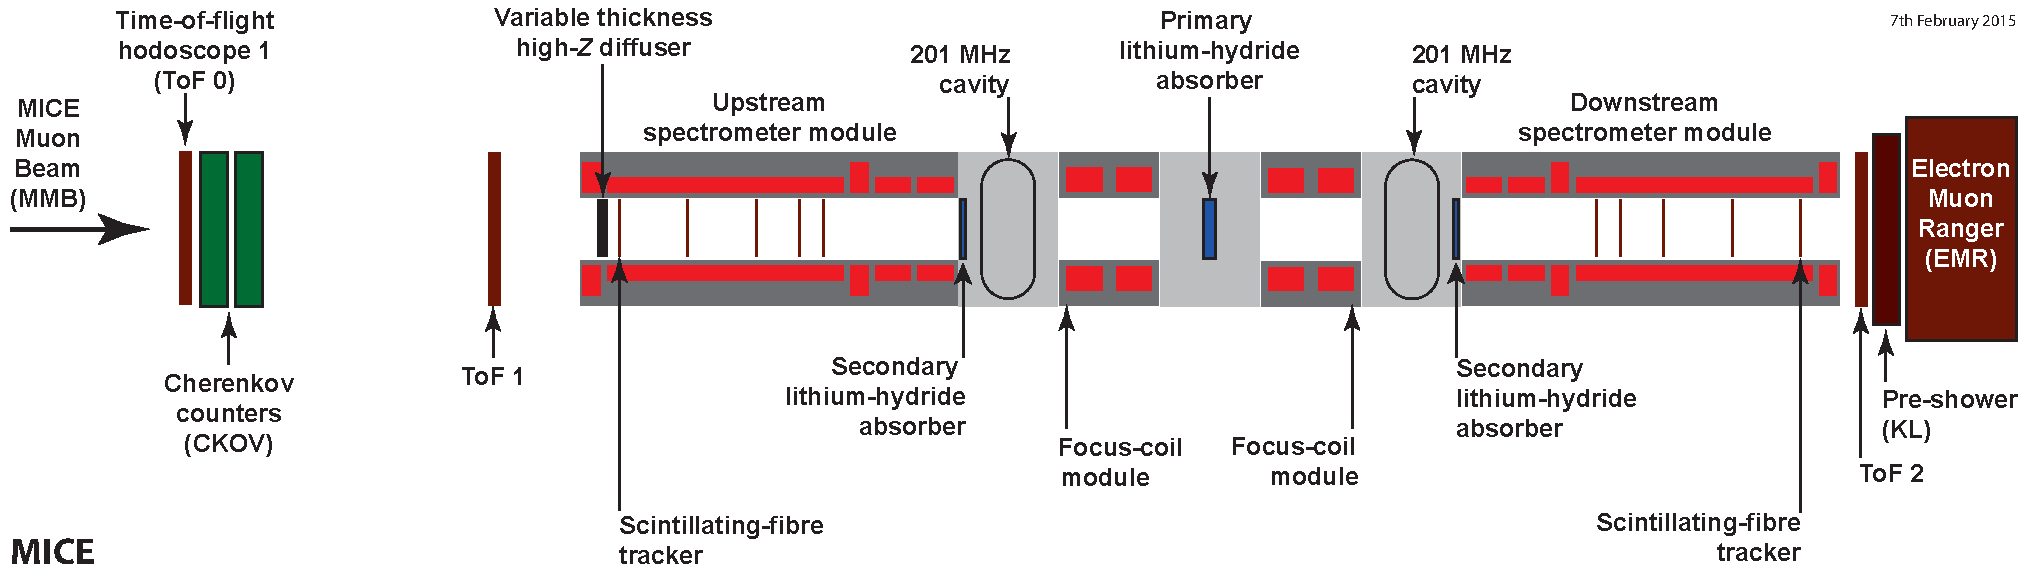
\includegraphics[width=.95\textwidth]{./Cooling-demo.pdf}
 % Cooling-demo-labels .pdf: 976x277 pixel, 72dpi, 34.43x9.77 cm, bb=0 0 976 277
 \caption{Schematic view of the MICE experiment.}
 \label{mice}
\end{figure}

MICE will measure the normalised transverse emittance $\epsilon_N$ with a precision of 
$\sigma_{\epsilon_N}/\epsilon_N \sim 0.1 \%$ when $6\%$ cooling effect is  expected for a muon beam with a nominal momentum
of $200 \ MeV/c$ and 4D normalised emittance $\epsilon_N = 5.8 \ \pi~mm~rad$.

\subsection{Electron-Muon Ranger (EMR)}
EMR is a fully active scintillator detector. It can be classified as tracking calorimeter, since its granularity allows for track
reconstruction. The primary purpose of the detector is to distinguish muons from their decay products, rejecting events in which
the muon decays in-flight along the cooling section \cite{ruslan}.  This allows for the selection of a muon beam with a contamination
below 1\%. The range of the muon track can be measured, providing an estimate of the momentum of the muon. 

The construction of the detector started in the early 2011 and in October 2013 the detector was fully commissioned with beam
during one month of a dedicated data-taking at RAL. In 2014 the detector was upgraded, including a replacement of the single-anode
photo-multiplier tubes and installation of a new high-voltage system.

\section{Design}
The EMR is built of triangular scintillator bars arranged in planes. 
% A drawing of one plane is shown on Figure~\ref{fig:emr_plane}.
One plane contains 59 bars and covers an area of 1.27~m$^2$. Each even bar is rotated by 180 degrees with respect to the odd one.
A cross-section of bars and their arrangement in a plane is shown in Figure~\ref{fig:bar_arrangement_in_a_plane}. With this
configuration there is no dead area for particles crossing a plane with angles less than 45 degrees from the beam axis.

\begin{figure}[htp!]
 \centering
 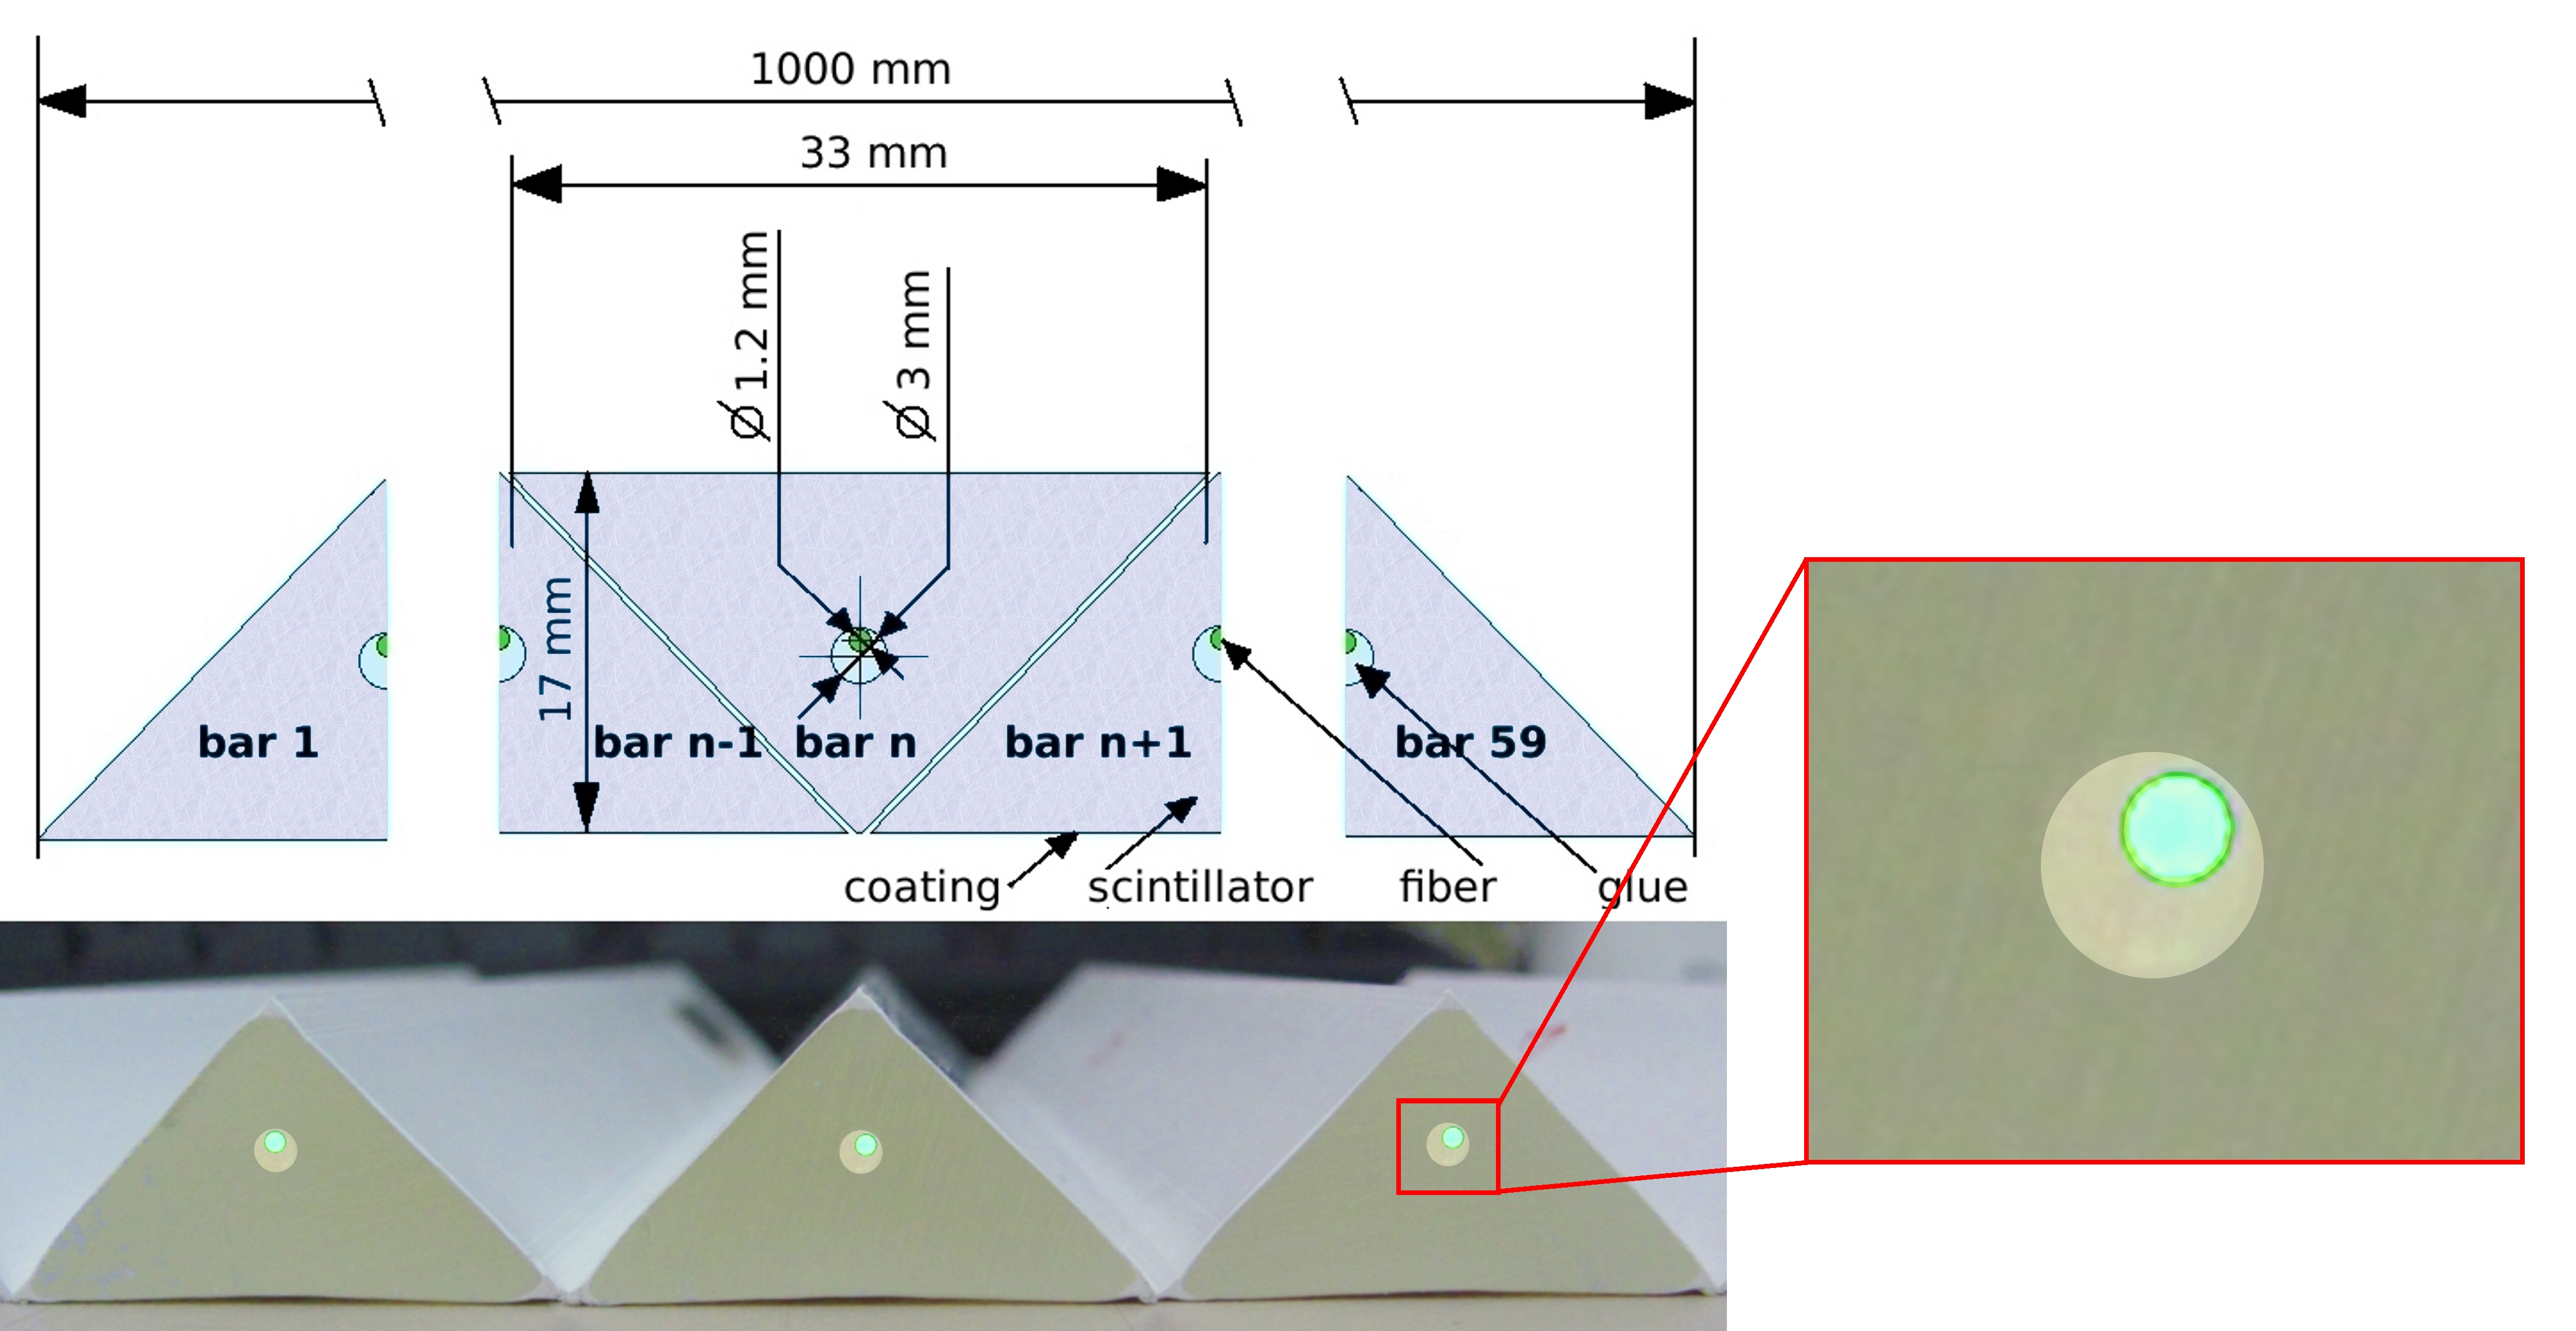
\includegraphics[width=0.9\textwidth]{./bar_arrangement_in_a_plane}
 \caption[EMR bar cross-section and plane arrangement]{EMR bar cross-section and bars arrangement in a plane. There are 59 bars per plane.}
 \label{fig:bar_arrangement_in_a_plane}
\end{figure}


The light, produced when a particle crosses a bar, is collected by a wave-length shifting (WLS) fiber glued inside the bar. 
At both ends of a bar the WLS fiber is coupled to a clear fiber that transfers the light to a photo-multiplier
(PMT). The clear fibers are protected with rubber sleeves and packed in aluminum fiber boxes as drawn in Figure 
\ref{fig:clear_fiber_package}. In order to reduce the bending radius, which affects light attenuation, each fiber has an individual
length. The two bunches of clear fibers coming from the two sides of a plane are glued into different types of connectors.
One is designed to match a multi-anode PMT, when the other one matches a single-anode PMT.

\begin{figure}[ht]
 \centering
 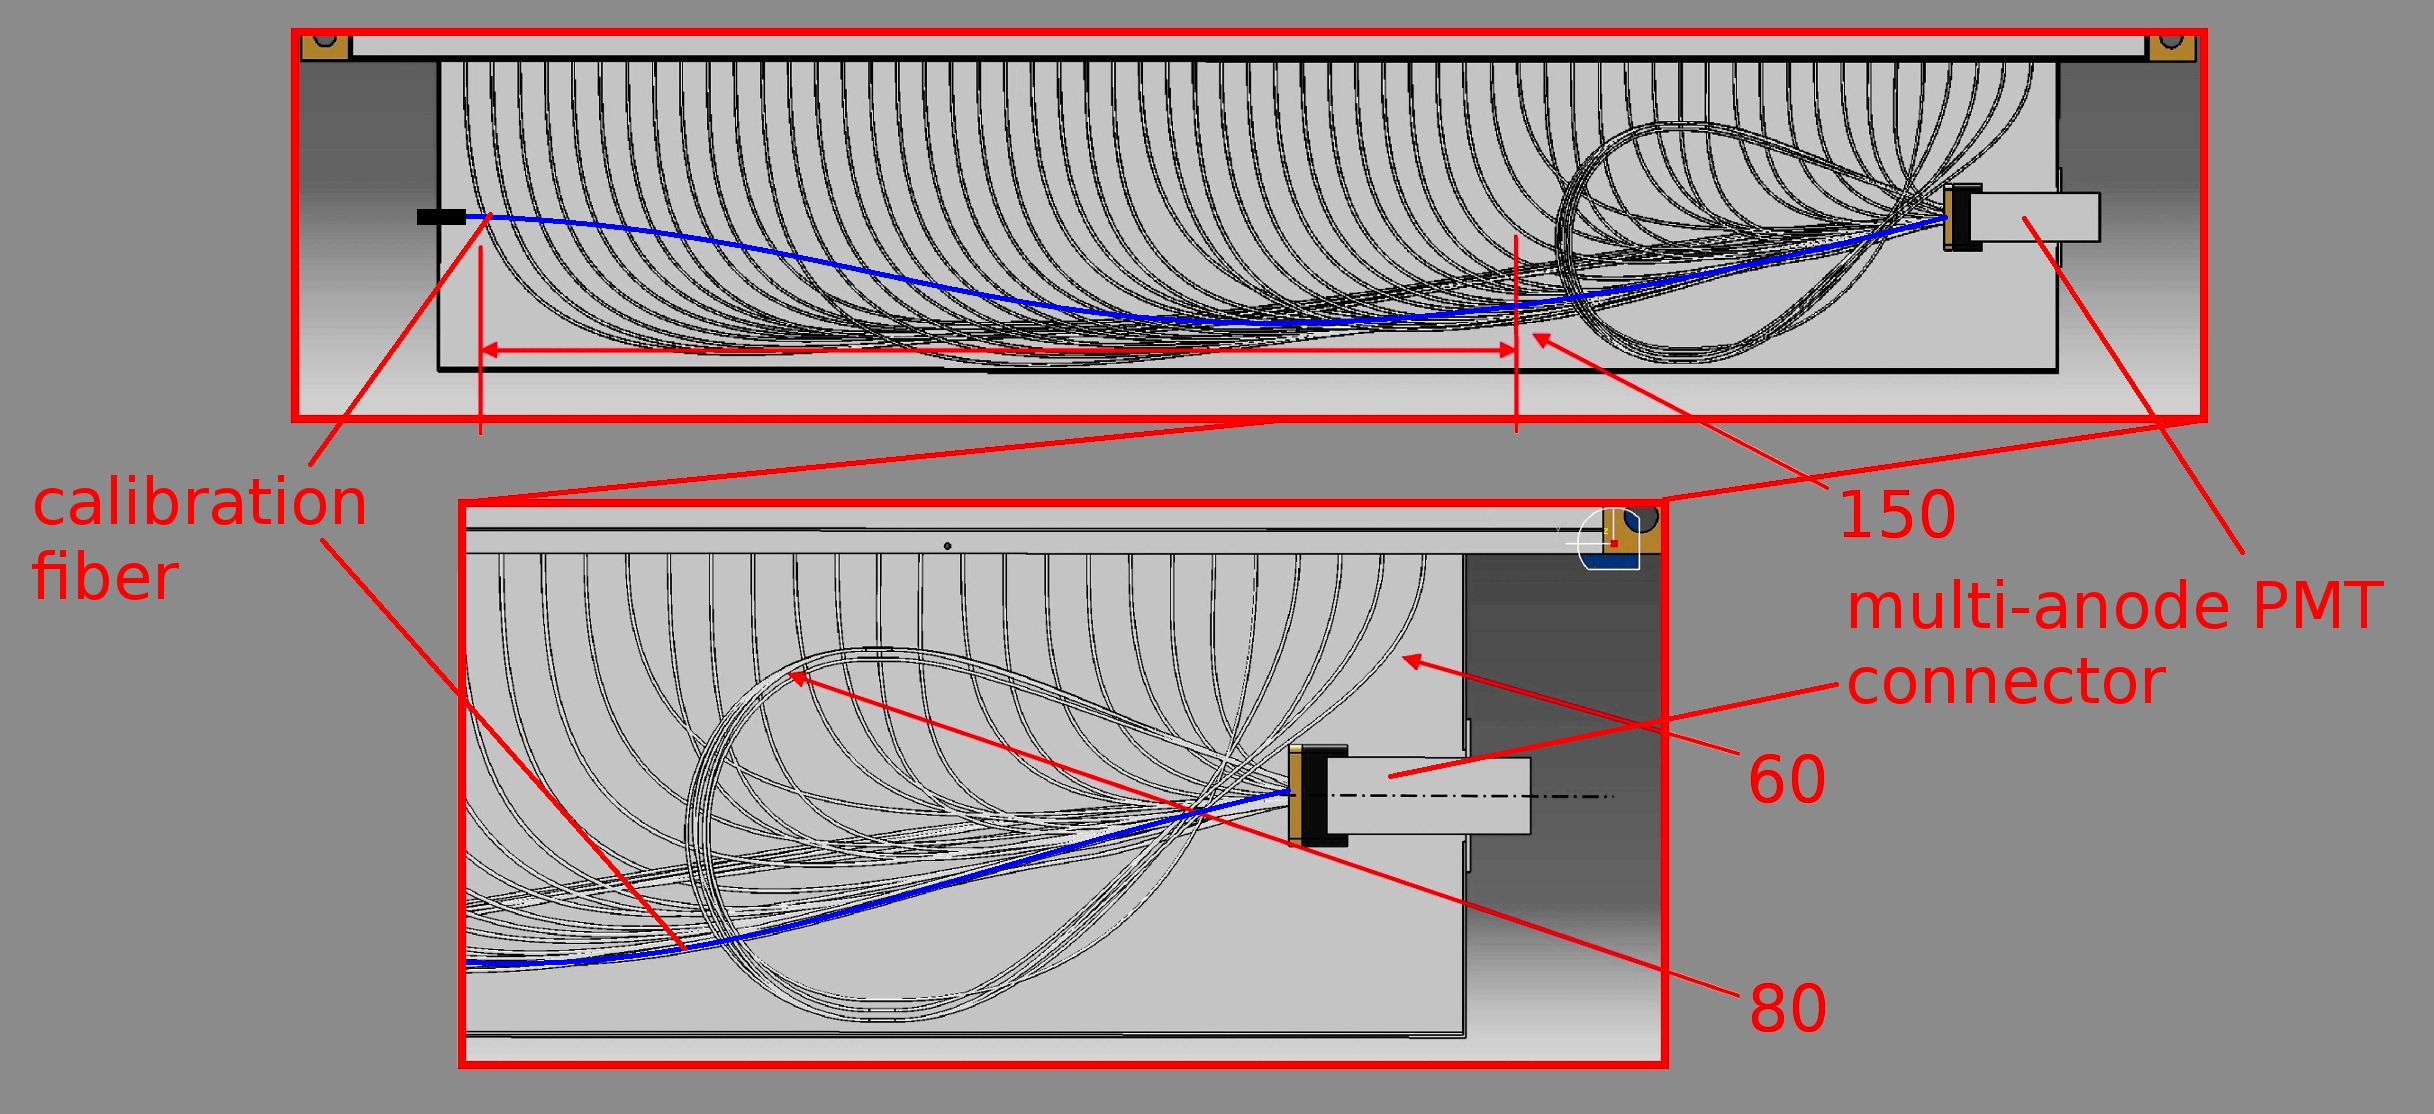
\includegraphics[width=0.95\textwidth]{./clear_fiber_package}
 \caption[A package of clear fibers in a fiber box]{ A package of clear fibers in a fiber box. Multi-anode PMT connector is shown.
 The fiber box for a single-anode PMT connector has similar structure. The last 5 fibers are looped in order to have largest possible
 bending radius. The bending radius of some of the fibers is indicate in red. The calibration fiber is also shown. }
 \label{fig:clear_fiber_package}
\end{figure}

\begin{figure}[htb]
 \centering
 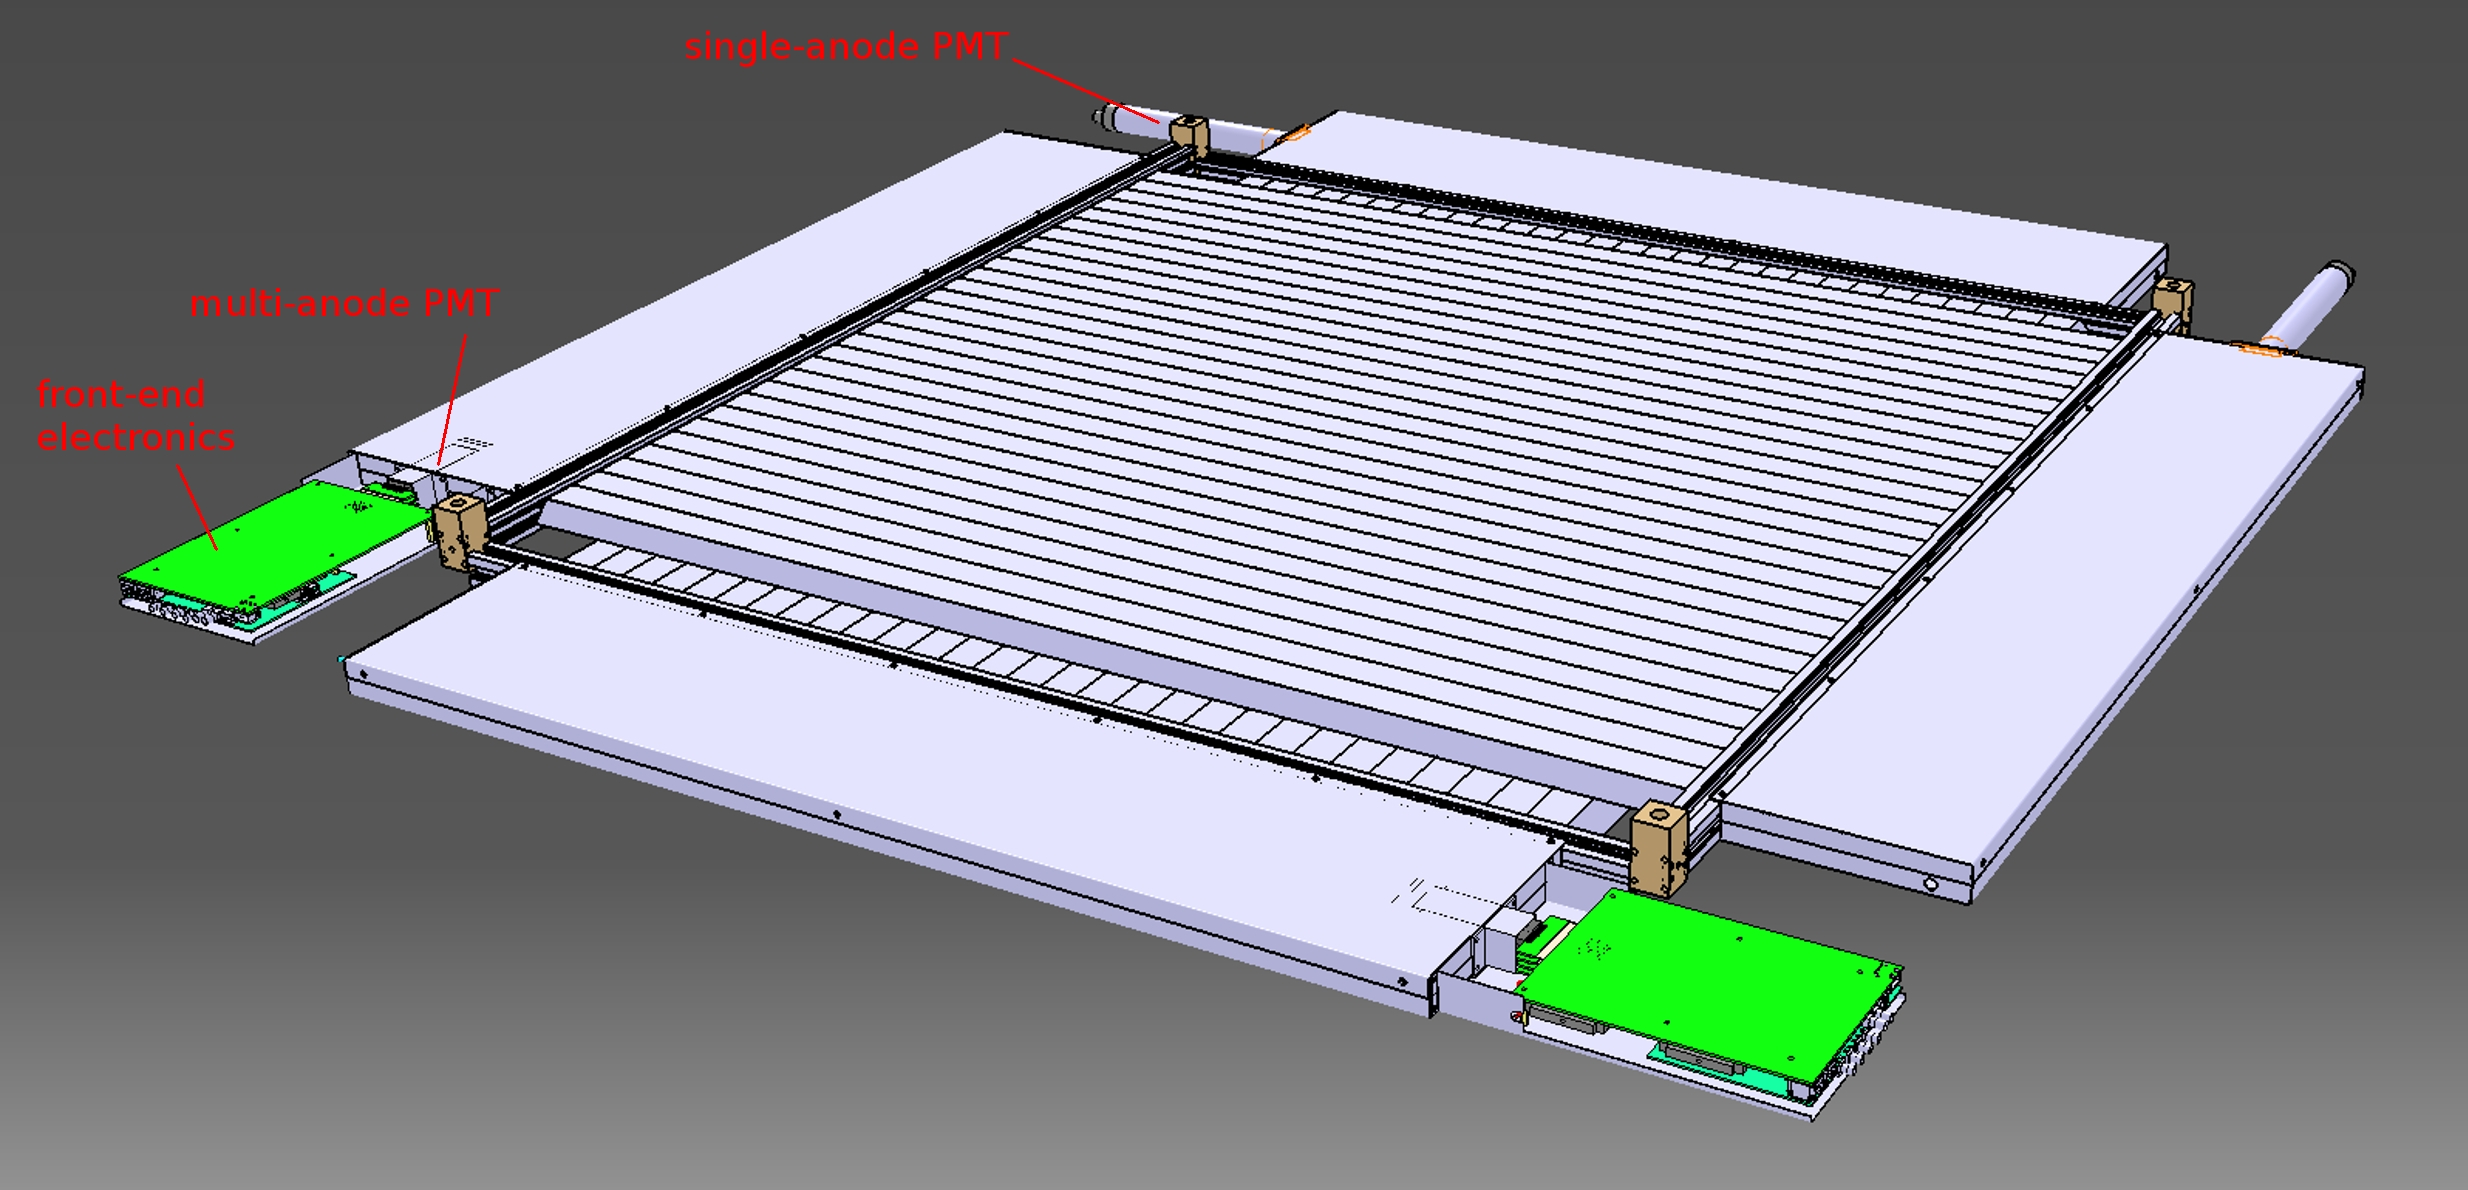
\includegraphics[width=0.85\textwidth]{./emr_module}
 \caption[CAD drawing of one EMR module]{CAD drawing of one EMR module made of X and Y planes. There are two front-end boards per module.}
 \label{fig:emr_module}
\end{figure}
\begin{figure}[htp!]
 \centering
%  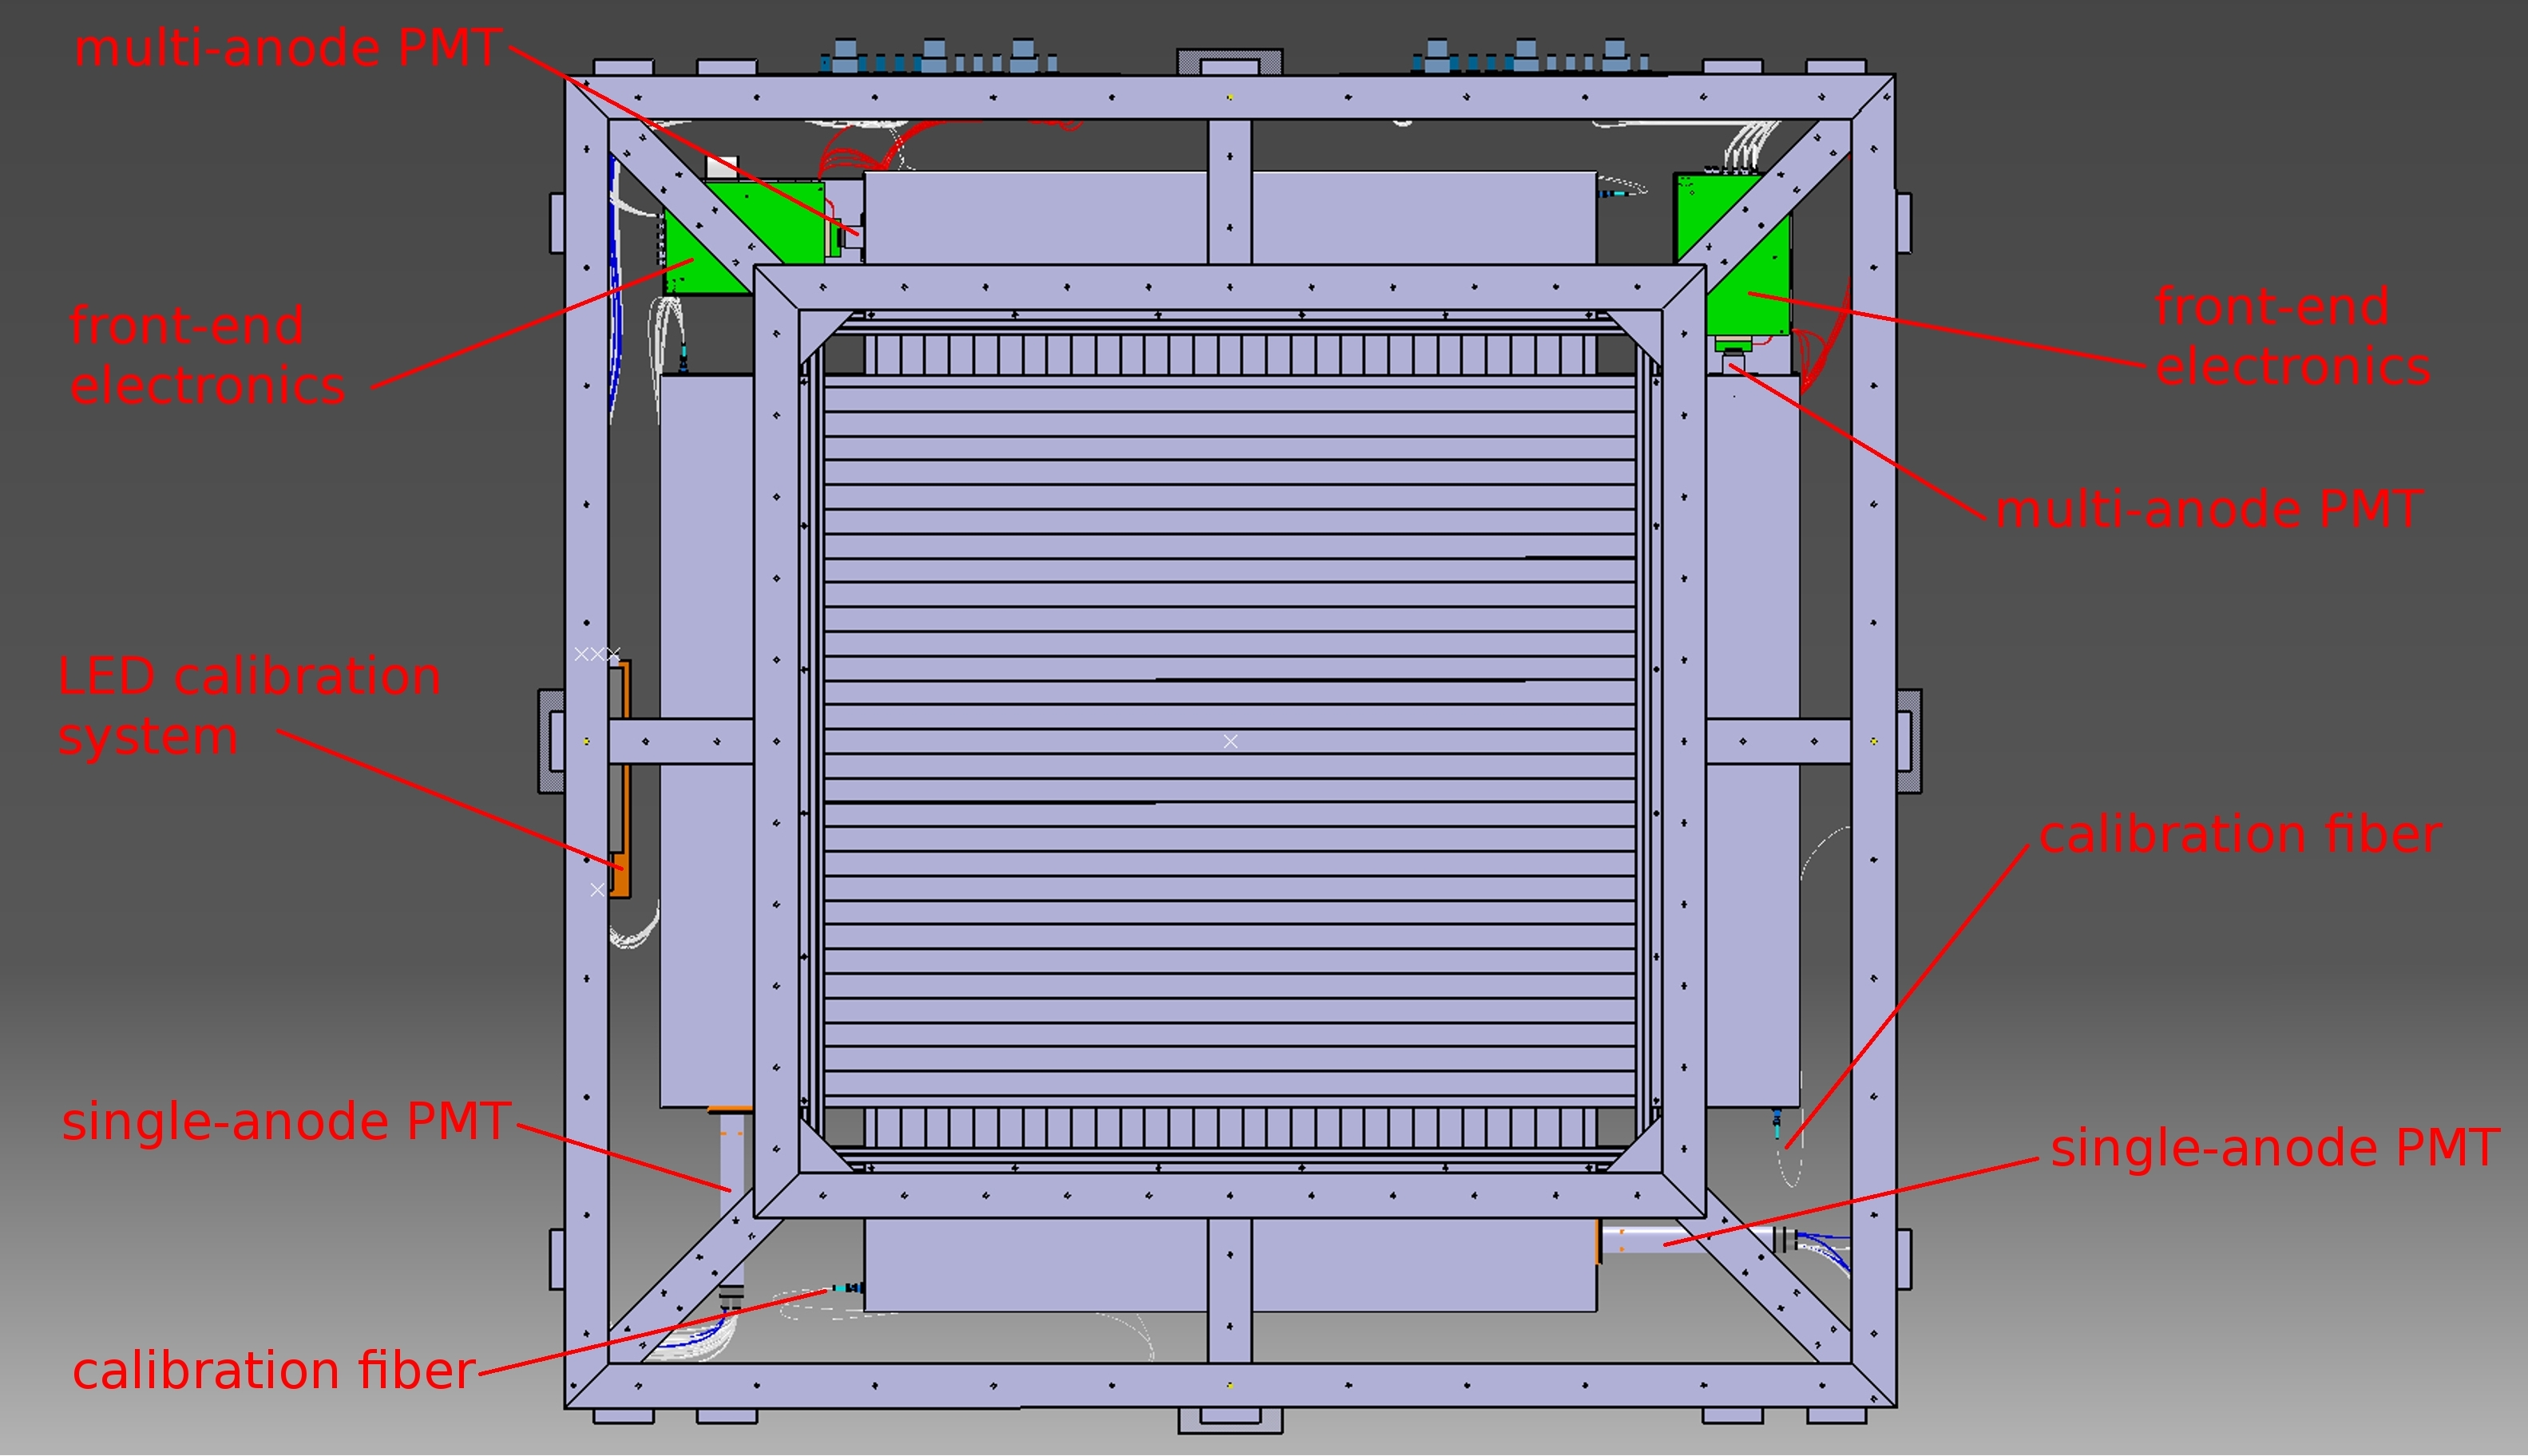
\includegraphics[width=\textwidth]{./emr_cad_model_2}\\
 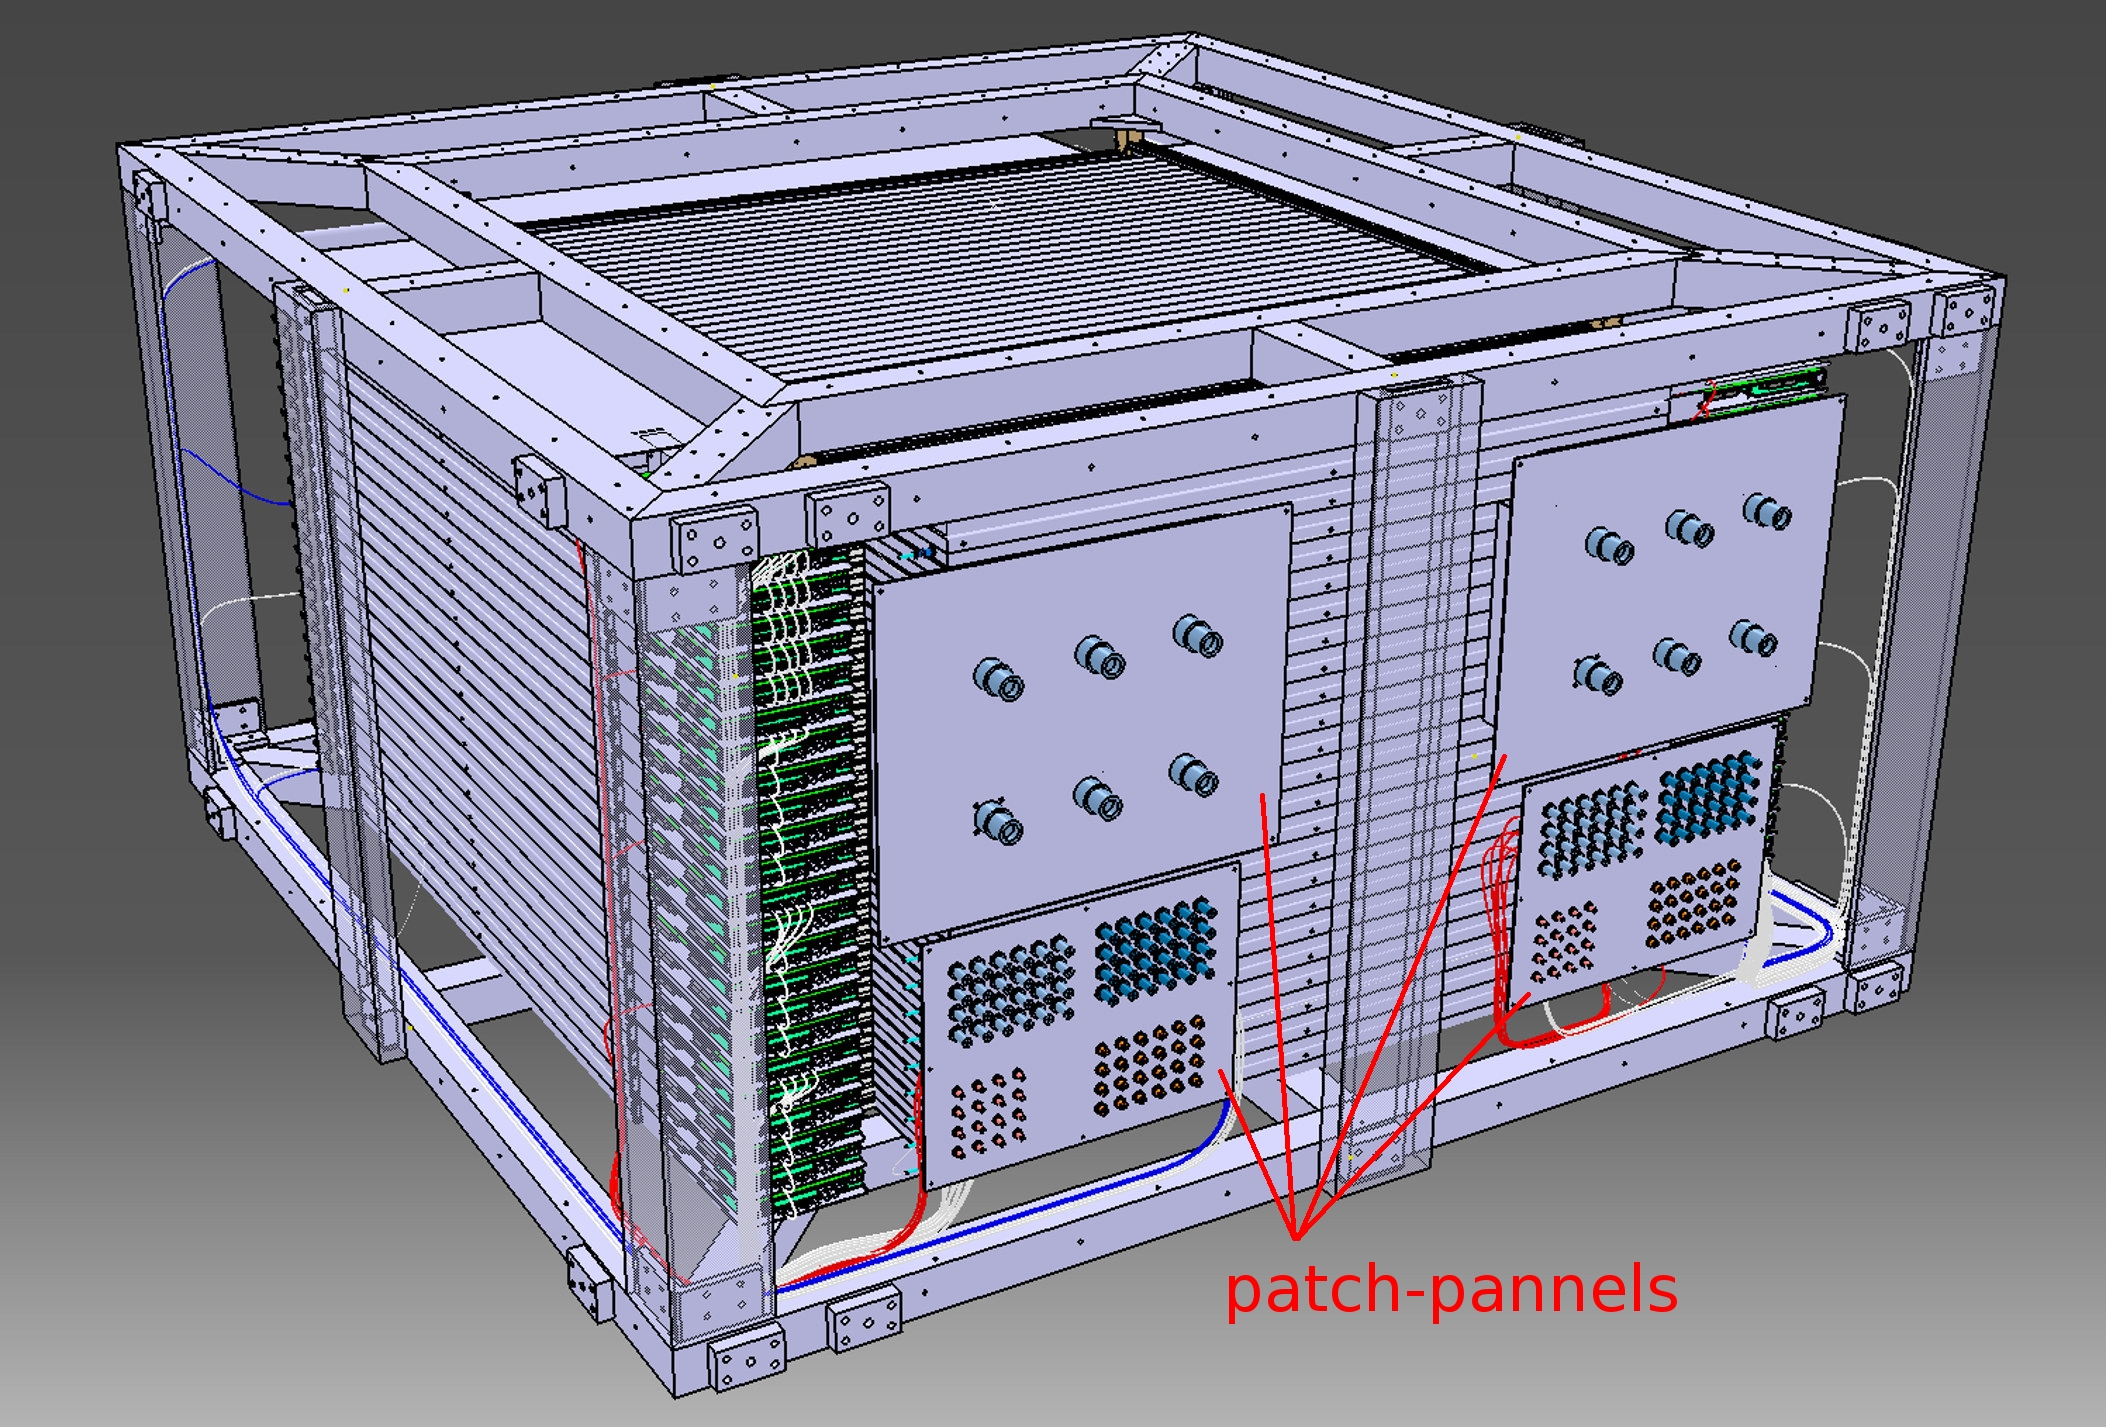
\includegraphics[width=0.75\textwidth]{./emr_cad_model_1}
 \caption[CAD drawing of the EMR detector]{CAD drawing of the complete EMR detector. The external protective panels are not shown.}
 \label{fig:emr_full_cad_model}
\end{figure}

Two planes attached to each other via aluminum profiles form a rigid structure called module (Figure~\ref{fig:emr_module}). 
The full detector contains 24 modules as shown in Figure~\ref{fig:emr_full_cad_model}. Panels cover all sides of the detector
in order to insure a light-tightness. The signal coming from each multi-anode PMT is read-out and processed by a front-end board
attached directly to the fiber box as shown in Figure \ref{fig:emr_module}. The single anode PMTs is equipped whit a
voltage divider and the analog signal is sent outside the detector for digitization.

A calibration system was installed inside the enclosure of the detector in order to monitor the drift of the gain and the quantum
efficiency of the PMTs. This system is made of a LED driver distributing light homogeneously to 100 fiber. Each fiber box is
connected to one of the calibration fibers through a dedicated connector. Inside a fiber box a clear fiber connects the calibration
fiber to the PMT (see Figure \ref{fig:clear_fiber_package}).

All cables inside the detector are feed through four patch-panels. There are 96 high-voltage, 6 low voltage, 48 analog, 48 digital,
and one configuration cables in total. A support frame is designed to withhold the full weight of the sensitive volume with electronics
($\sim$ 1 tonne). In order to protect the front-end electronics from the magnetic field of the spectrometer solenoid, situated nearby
the detector, a shielding plate is mounted on the side of the detector that faces the beam. The total weight of the detector is almost
2.5 tonnes.

\subsection{Optical Elements}
The scintillator bars were manufactured at an extrusion facility at Fermilab~\cite{PlaDalmau:2001fr}. This facility also produced
scintillators of different shapes for other experiments like: DO preshower detector, MINOS~\cite{PlaDalmau:2001en},
Minerva~\cite{PlaDalmau:2005df}, SciBar (K2K/SciBoone), Star, Mayn Pyramid Mapping, Hall-B JLAB, T2K-ND280, Double-Chooz, Amiga
- Piere Auger. Each bar is 110~cm long, 1.7~cm high and 3.3~cm wide with 3~mm hole along the bar for a wavelength shifting fiber.
The scintillator is made of polystyrene pellets\footnote{Dow Styron 663 W} as base, 1\% PPO\footnote{scintillator, 2,5-diphenyloxazole,
C$_{15}$H$_{11}$NO} as primary and 0.03\% POPOP\footnote{wavelength shifter, 1,4-di-(5-phenyl-2-oxazolyl)-benzene, C$_{24}$H$_{16}$N$_{2}$O,
spectrum peaks at 410 nm (violet)} as secondary fluor. Each bar is coated with TiO$_2$ reflector in order to increase light collected by 
the WLS fiber. Light output of the scintillator was measured~\cite{PlaDalmau:2001fr} with a photo-multiplier (25\% quantum efficiency)
and it is around 17 photo-electrons. 

The WLS fiber glued inside the bar is a double cladding 1.2~mm in diameter fiber, produced by Saint-Gobain Crystals~\cite{saintgobain}.
The core material of the fiber is polystyrene with acrylic cladding. It has very large numerical aperture of 0.58 compared to 0.2-0.3
of graded-index multi-mode fiber used in data communications. Trapping efficiency is 3.5\%. The light is absorbed in the blue part of
the visible spectrum and re-emitted in green. 

The clear fiber, used to transfer light from the ends of scintillator bar to the PMTs, is a 1.5mm multi-cladding fiber produced by 
Kuraray~\cite{kuraray} with special structure (S-type) that allows for better rigidity against bending. The aperture of this fiber matches
to the one of WLS fiber so that insertion loss is minimal.

A special connector was designed to couple the clear fiber to the WLS fiber (see Figure~\ref{fig:fiber_connectors_cad}). It has a small
cylindrical enlargement which is meant to be filled with glue to fix the fiber in the connector. This configuration helps
to avoid crimping the fiber since a sharp edge of the connector would easily damage it. As shown in Figure~\ref{fig:fiber_connectors_cad}
the retaining clip (B) is screwed into the wavelength shifting fiber connector (A) so that clear fiber connector can be easily and safely
attached. All these peaces are non-standard and could not be found on a market, therefore a special mold was designed to produce them using
injection molding technique. 

\begin{figure}[htp!]
 \centering
 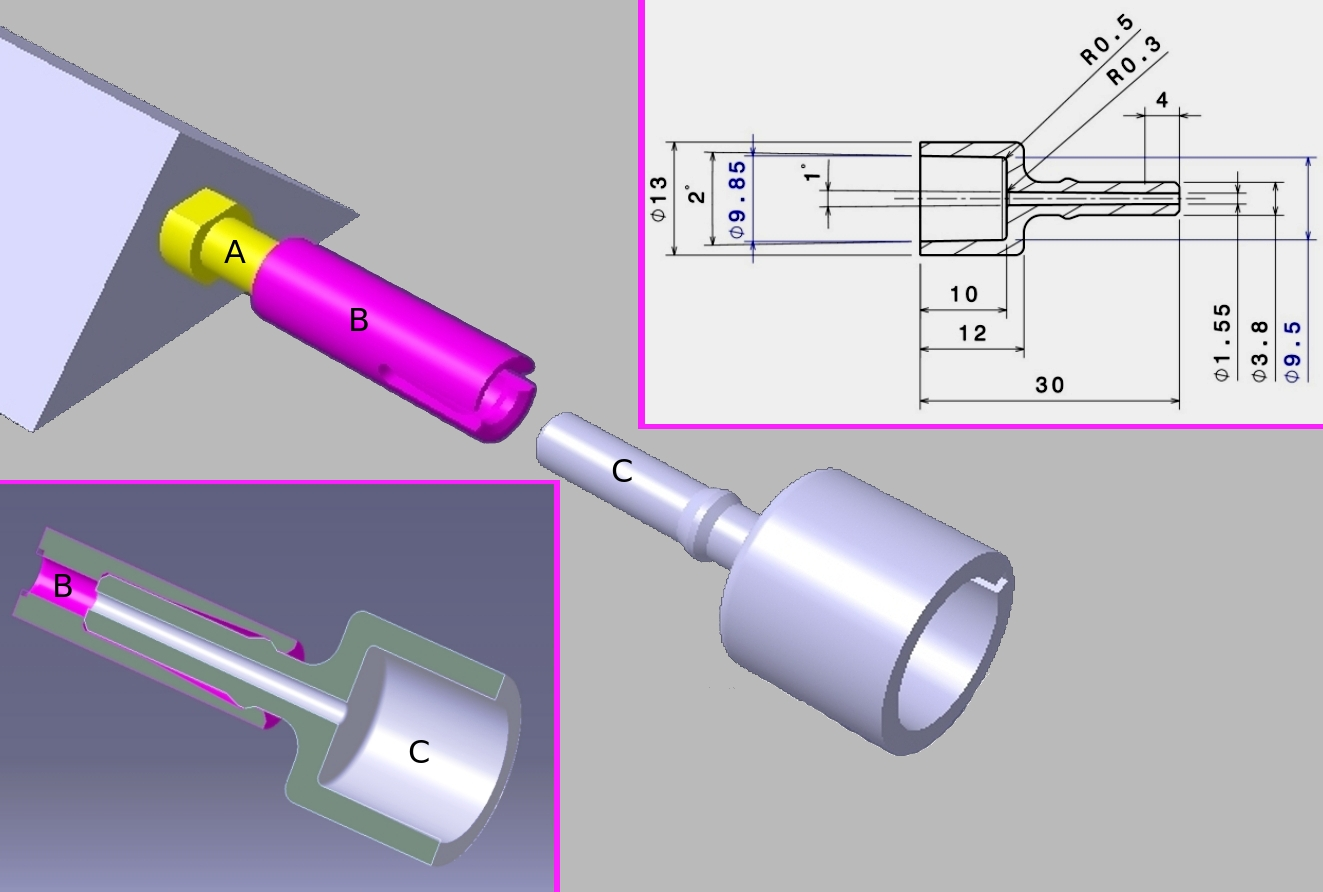
\includegraphics[width=0.8\textwidth]{./fiber_connectors_cad}
 \caption[Clear fiber connector]{clear fiber connector (C) is attached to the wavelength shifting fiber connector (A) via retaining clip (B).}
 \label{fig:fiber_connectors_cad}
\end{figure}

\begin{figure}[htp!]
 \centering
 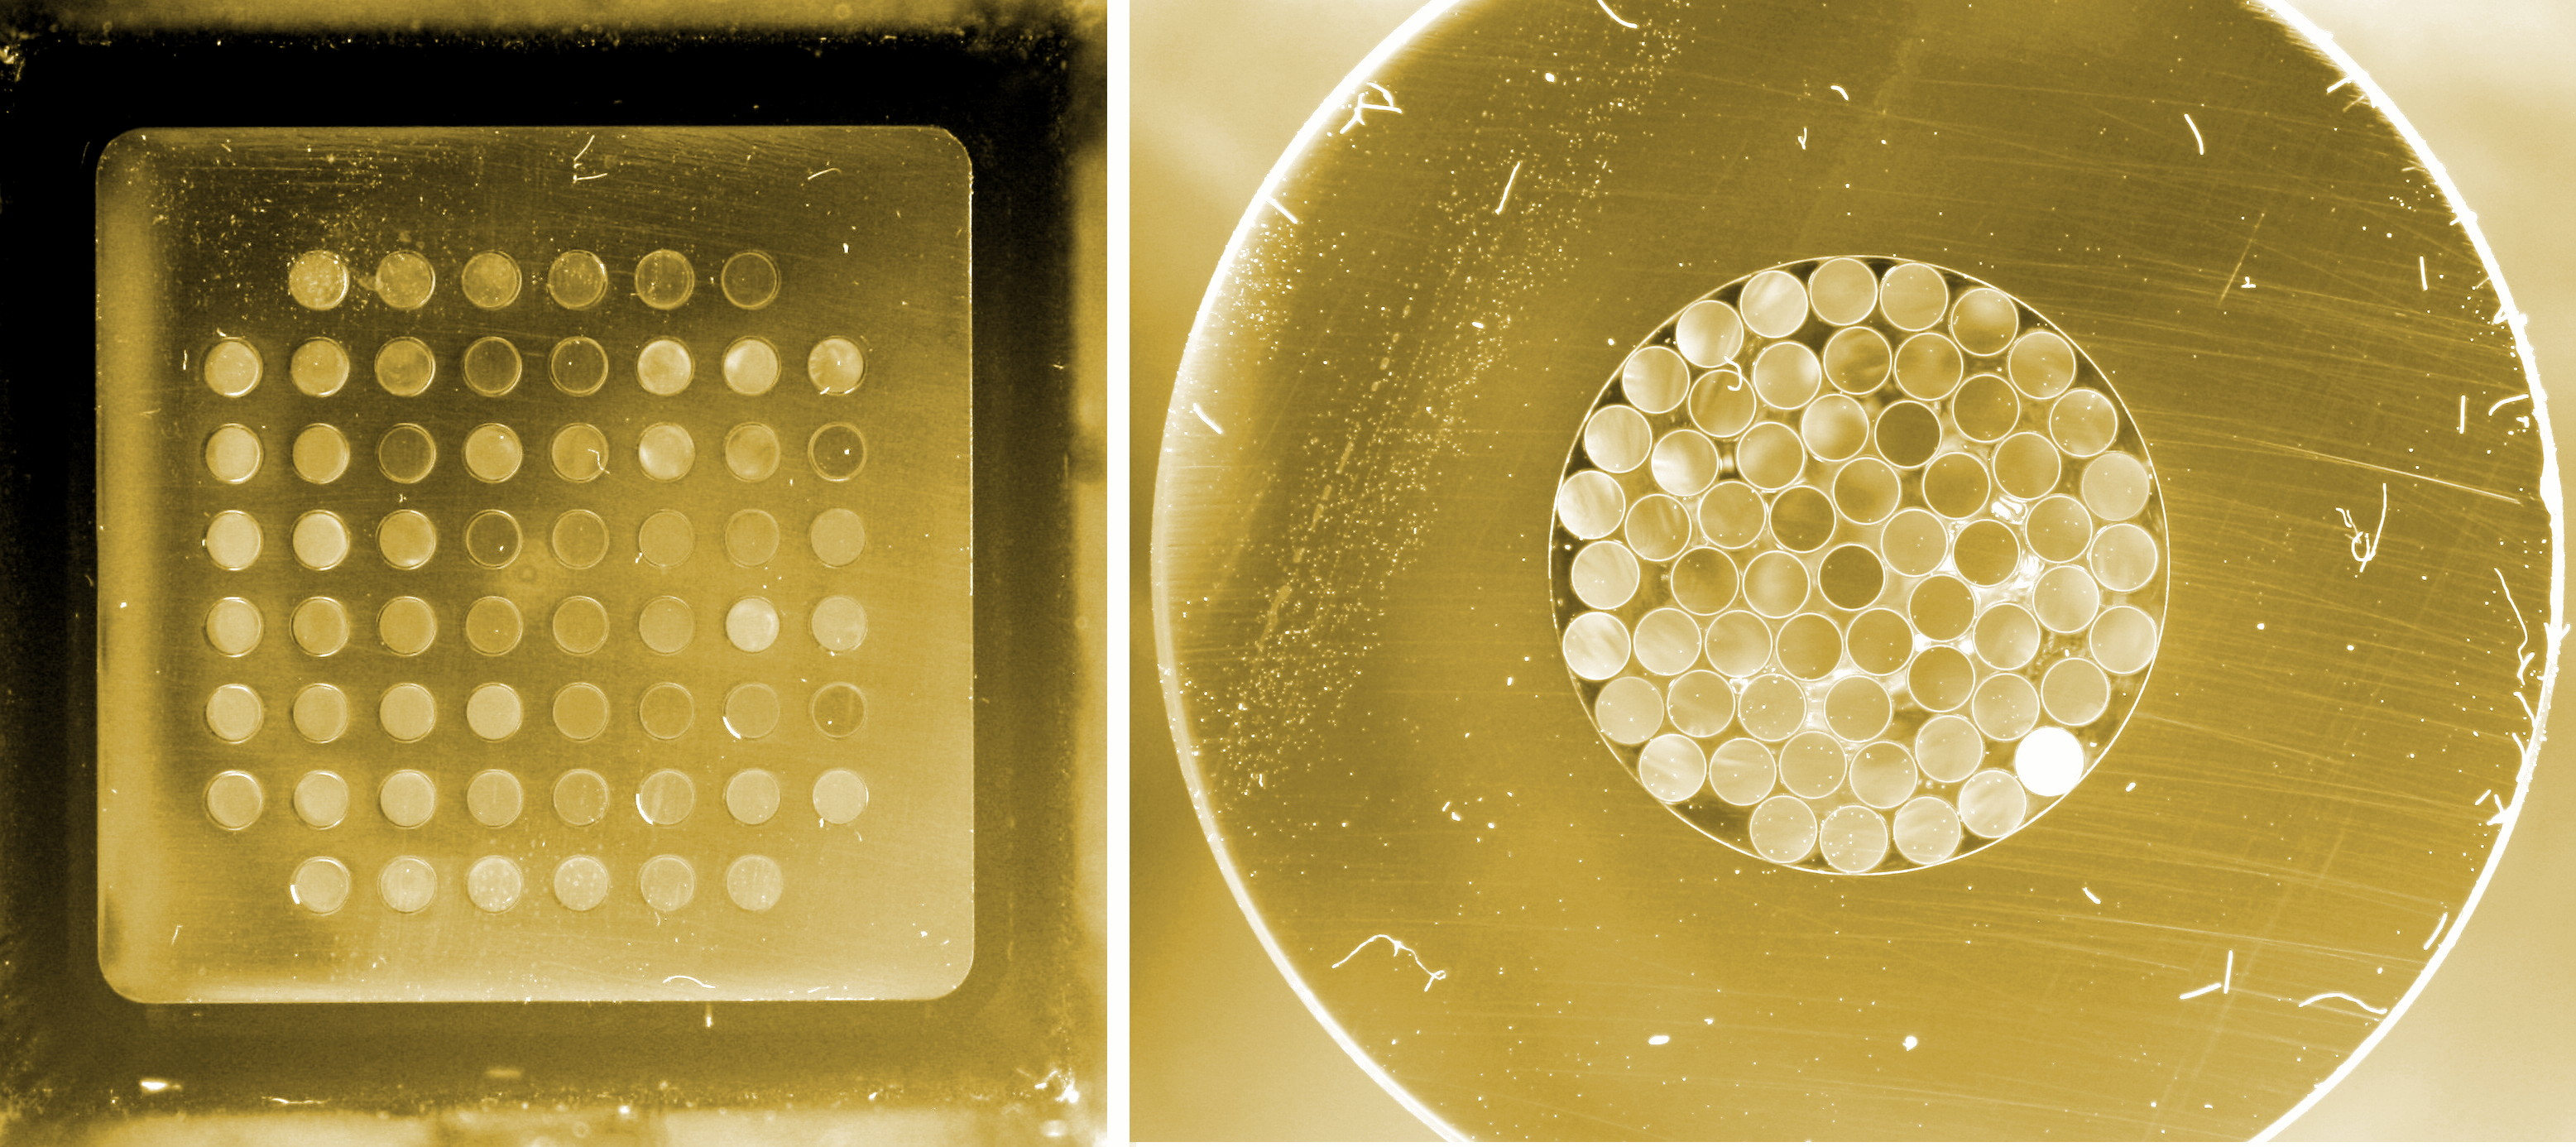
\includegraphics[width=0.85\textwidth]{./pmt_connectors.JPG}
 \caption[PMT connectors]{{\bf Left:} multi-anode PMT connector. {\bf Right:} single-anode PMT connector.}
 \label{fig:pmt_connectors}
\end{figure}

\subsection{Photo-detectors}
As it was briefly mentioned earlier the EMR has a dual readout. Each scintillator plane is equipped with a multi-anode PMT, which collects
the light from the individual bars and a single-anode PMT which detects the integrated response of all bars in the plane. 
\begin{figure}[h]
 \centering
 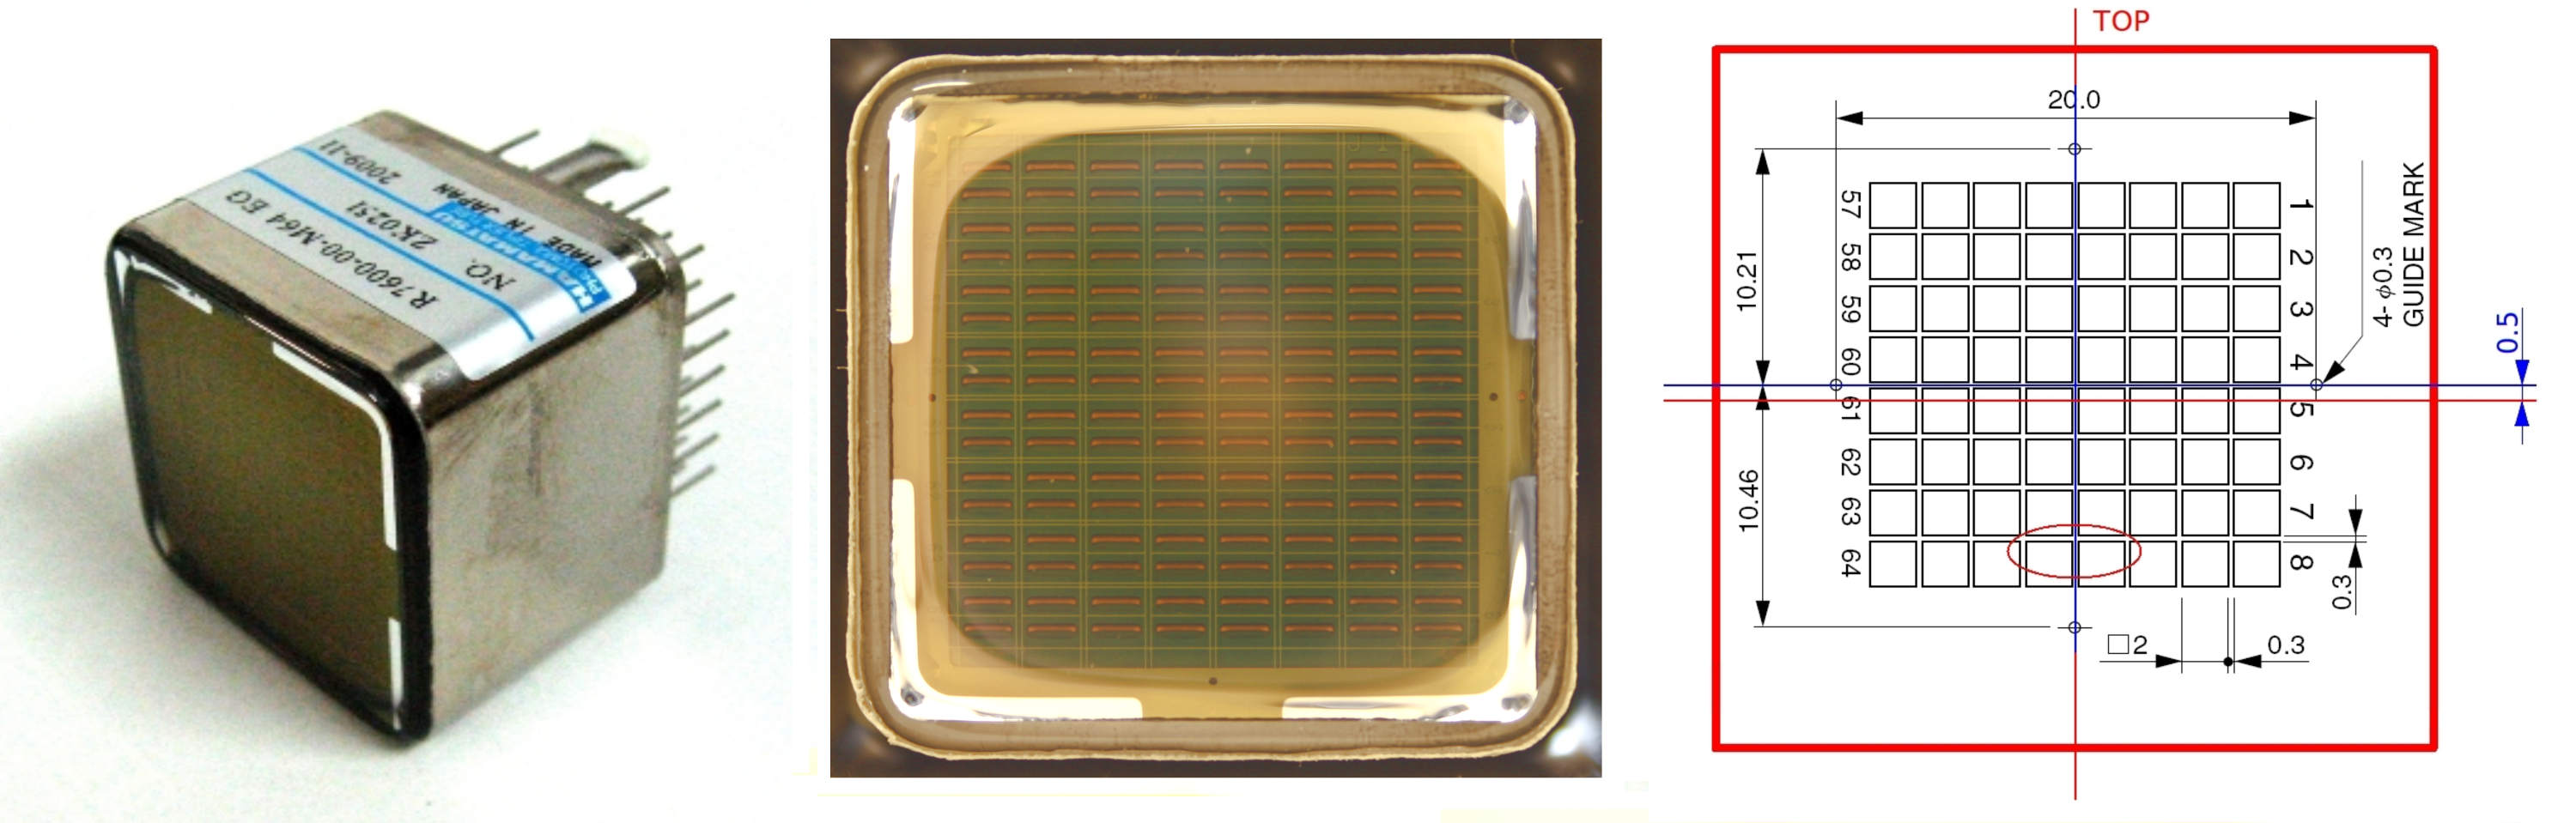
\includegraphics[width=\textwidth]{./mapmt}
 \caption[Multi-Anode PMT]{Multi-Anode PMT. {\bf Left:} photo. {\bf Center:} anode matrix. {\bf Right:} anode matrix dimensions.}
 \label{fig:mapmt}
\end{figure}
\begin{figure}[h]
 \centering
 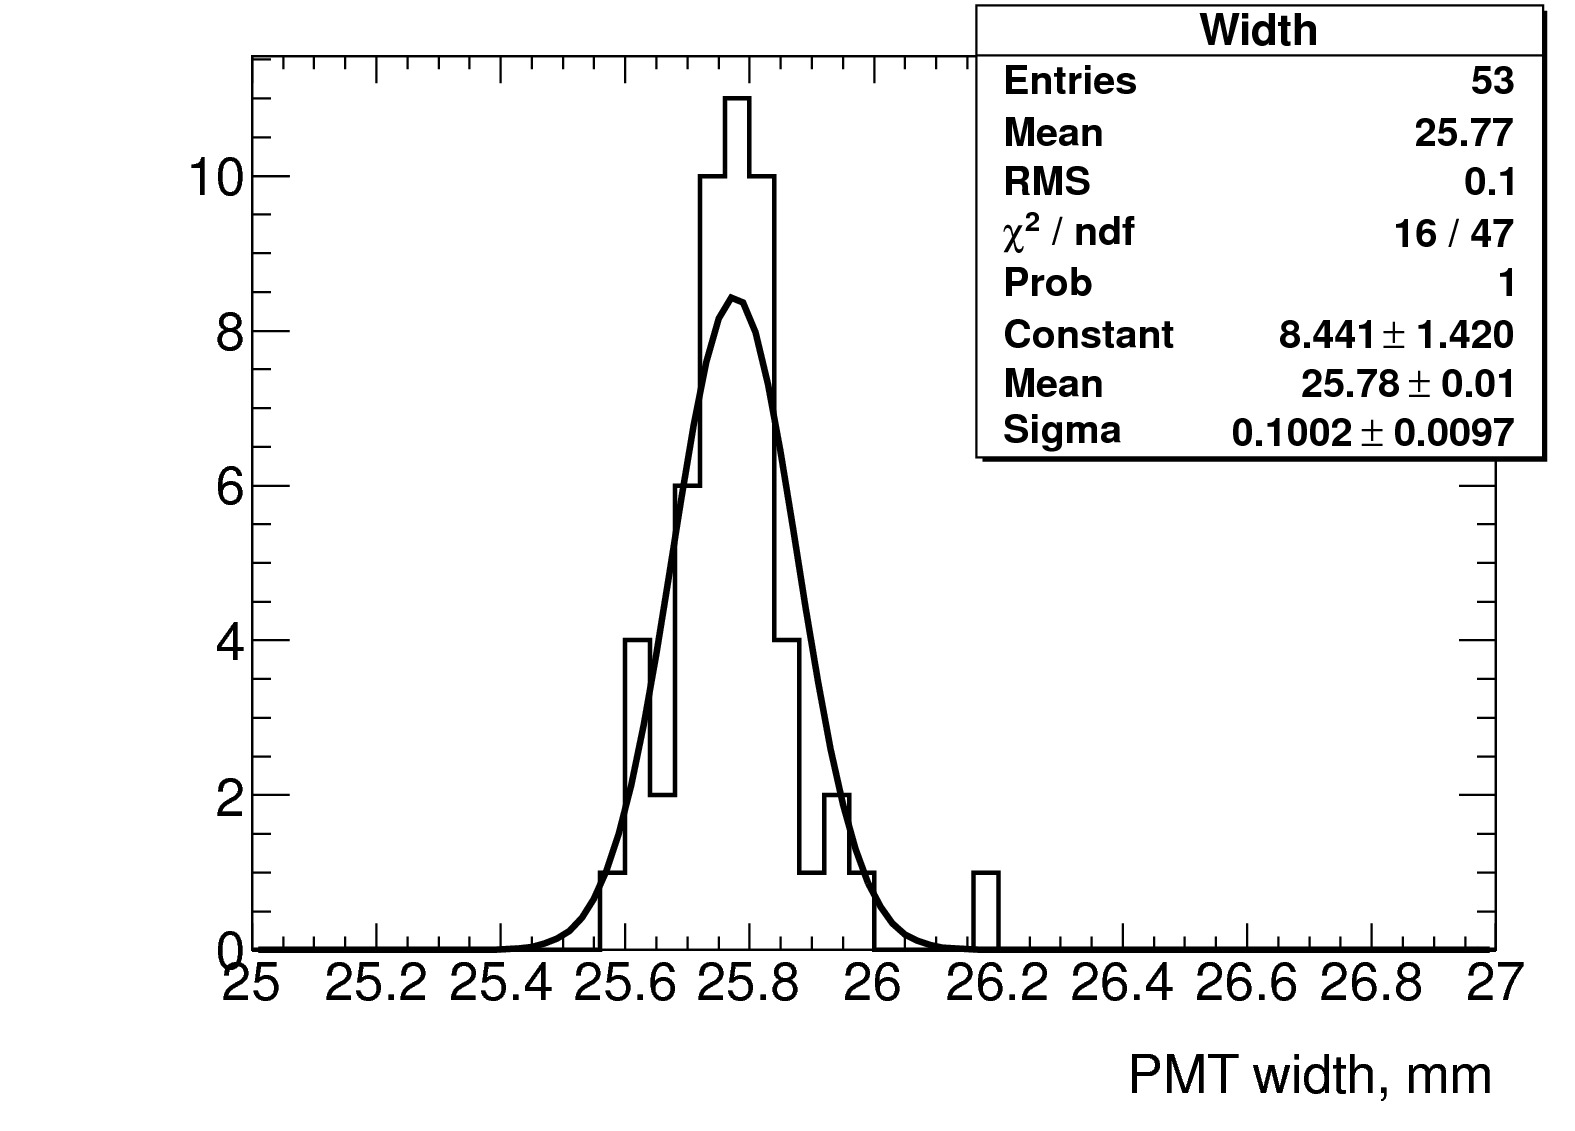
\includegraphics[width=0.45\textwidth]{./mapmt_width}
 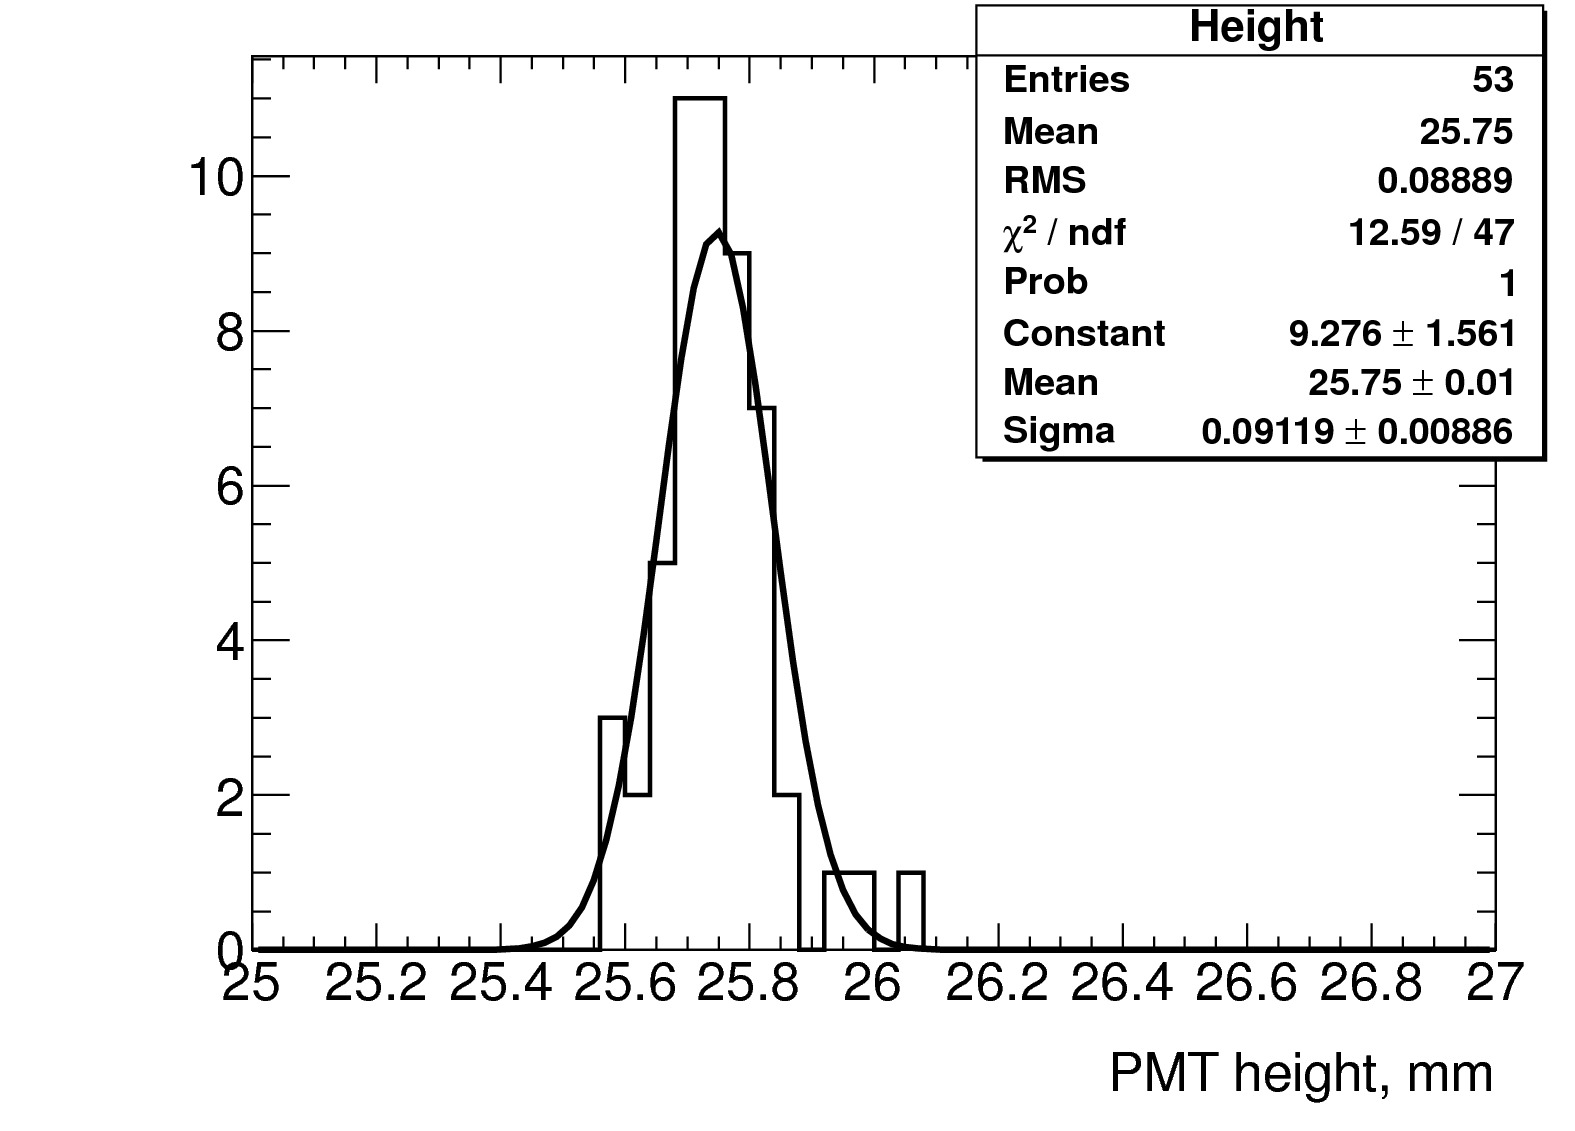
\includegraphics[width=0.45\textwidth]{./mapmt_height}\\
 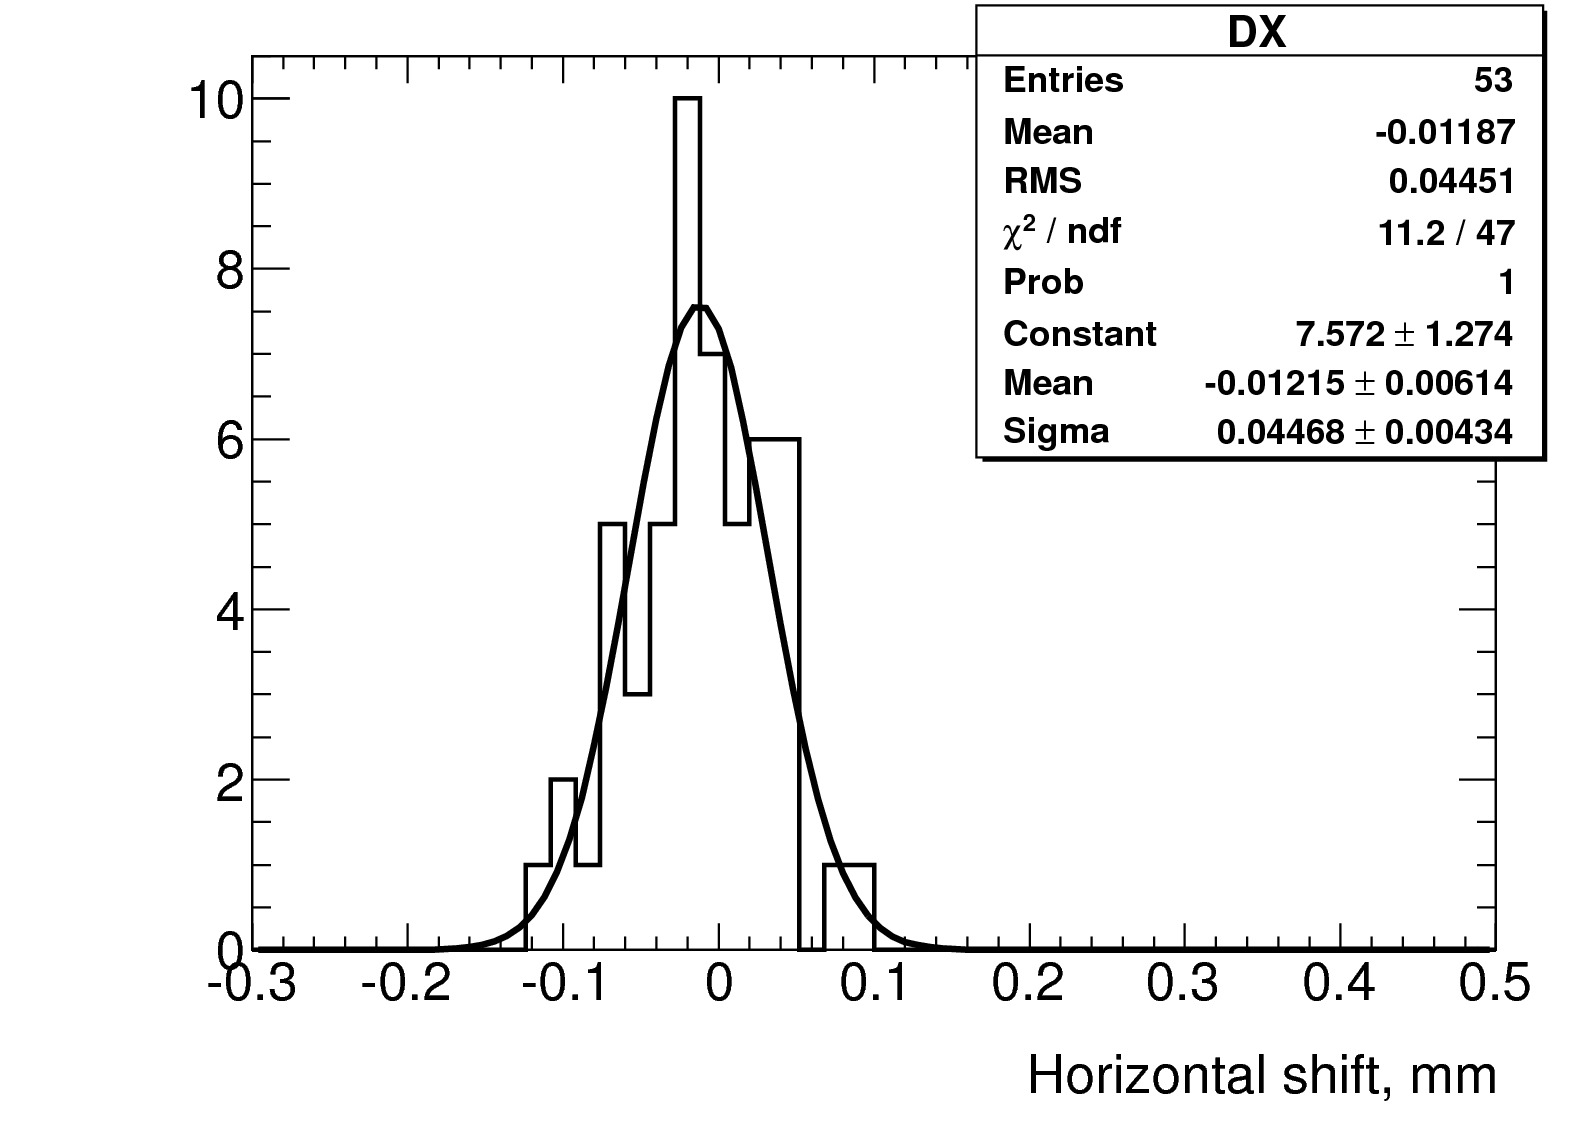
\includegraphics[width=0.45\textwidth]{./mapmt_horizontal_shift}
 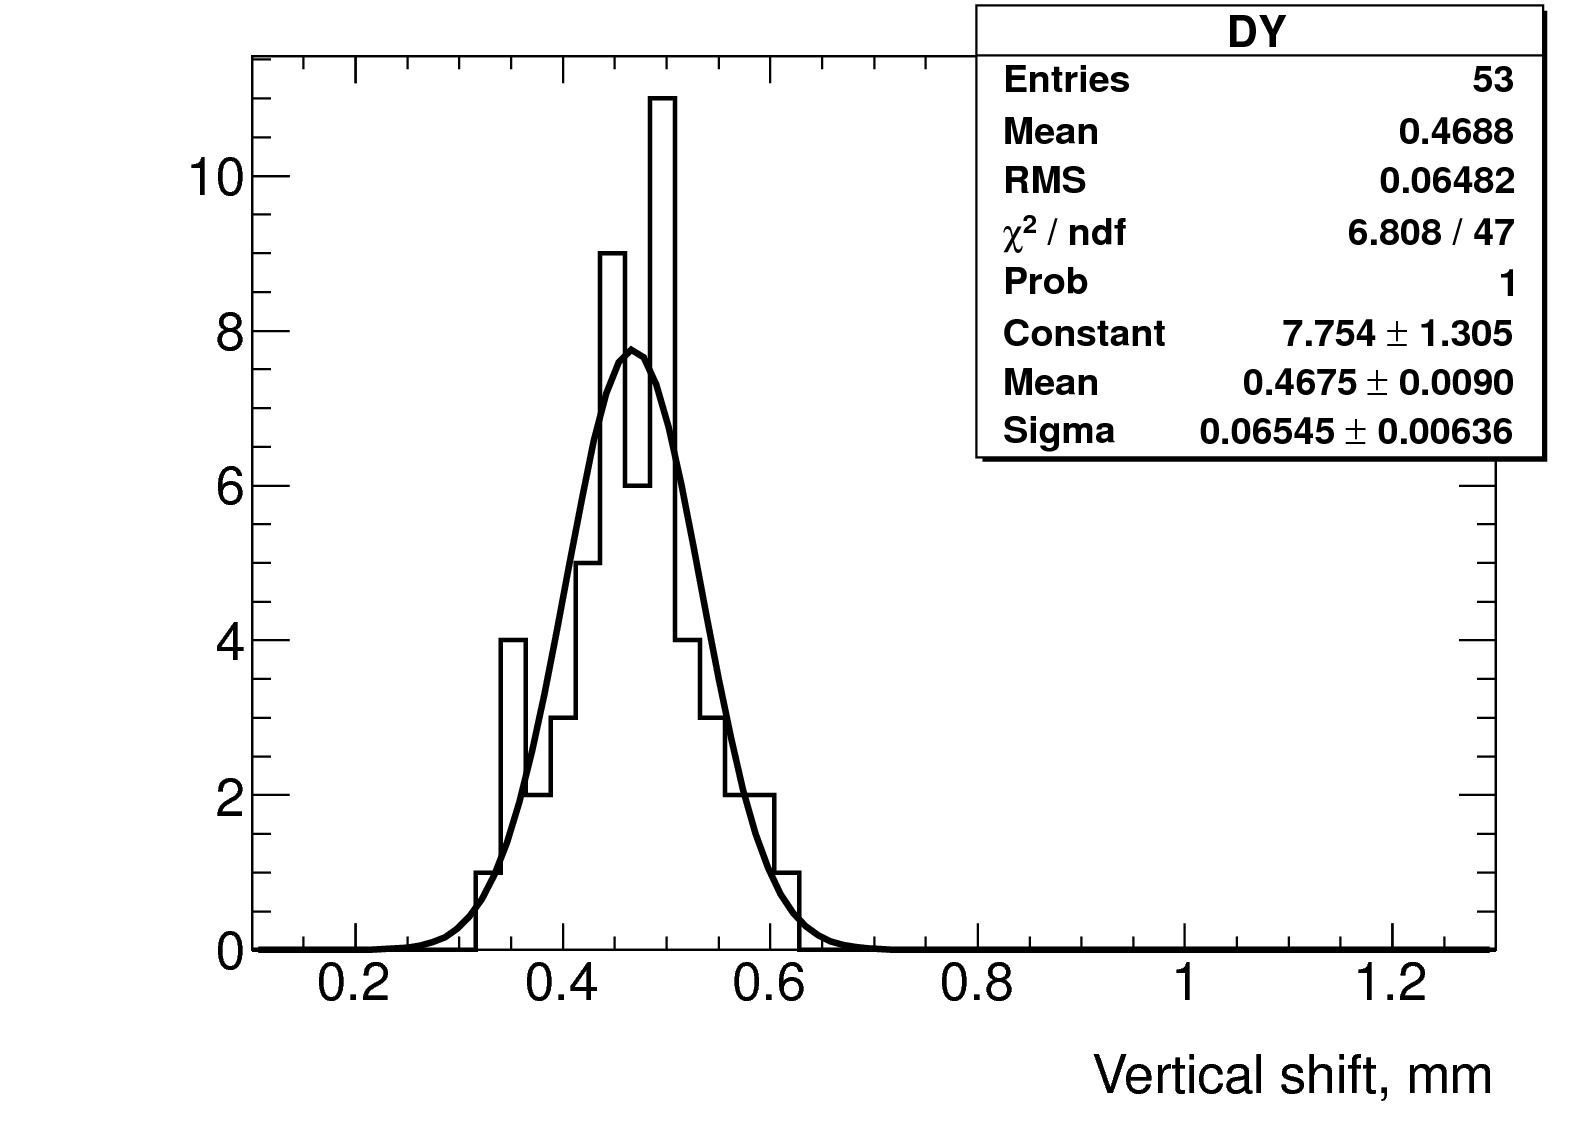
\includegraphics[width=0.45\textwidth]{./mapmt_vertical_shift}
 \caption[Distribution of Multi-Anode PMT dimensions]{Distribution of Multi-Anode PMT dimensions.}
 \label{fig:mapmt_dimensions}
\end{figure}

The multi-anode photo-multiplier tube (MAPMT) is a 64-channel PMT produced by Hamamatsu (model R5900-00-M64~\cite{hamamatsu_mapmt}, see
Figure~\ref{fig:mapmt}, left). The spectral sensitivity matches to the emission spectrum of the wavelength shifting fiber. It is 
placed in a $\mu$-metal tube  which serves as an additional shielding against the static magnetic filed. Inside the $\mu$-metal tube,
the PMT is aligned with respect to the fiber connector in such a way that each fiber shines only one
channel. Therefor it was important to measure all dimensions of the PMT and especially position of the anode matrix with respect to the
PMT case (Figure~\ref{fig:mapmt}, centre). Figure~\ref{fig:mapmt_dimensions} shows distributions of the measured dimensions (width and
height) and displacements of the anode matrix for 53 MAPMTs. It was found that on average the matrix is shifted by 0.5~mm upwards (see
Figure~\ref{fig:mapmt}, right and Figure~\ref{fig:mapmt_dimensions}, bottom right). This was taken into account in the design of the
MAPMT fiber connectors.

As for the MAPMTs, the single-anode photo-multiplier tube (SAPMT) is placed in a $\mu$-metal tube. The EMR detector was initially assembled
by reusing old SAPMTs, available after the disassembly of the HARP experiment \cite{harp}. These were 10 stage linear focused PMTs produced
by Philips (model XP2972). A special selection procedure was developed in order to select the best samples for the assembly of the detector
\cite{philips}. In 2014, during the upgrade of the detector, all Philips SAPMT were replaced by new SAPMTs produced by Hamamatsu (model R6427
\cite{hamamatsu_mapmt}).

\subsection{Electronics Layout}
In MICE the spill is defined as the period when the target crosses the ISIS proton beam. The maximum spill repeating rate allowed by the
MICE target system is $\sim 0.75 \ Hz$. The overall principle of the MICE Data Acquisition (DAQ) system is that during the spill the
accumulated digital data is kept in local memory buffers and the readout is performed only at the end of the spill.

\begin{figure}[htp!]
 \centering
 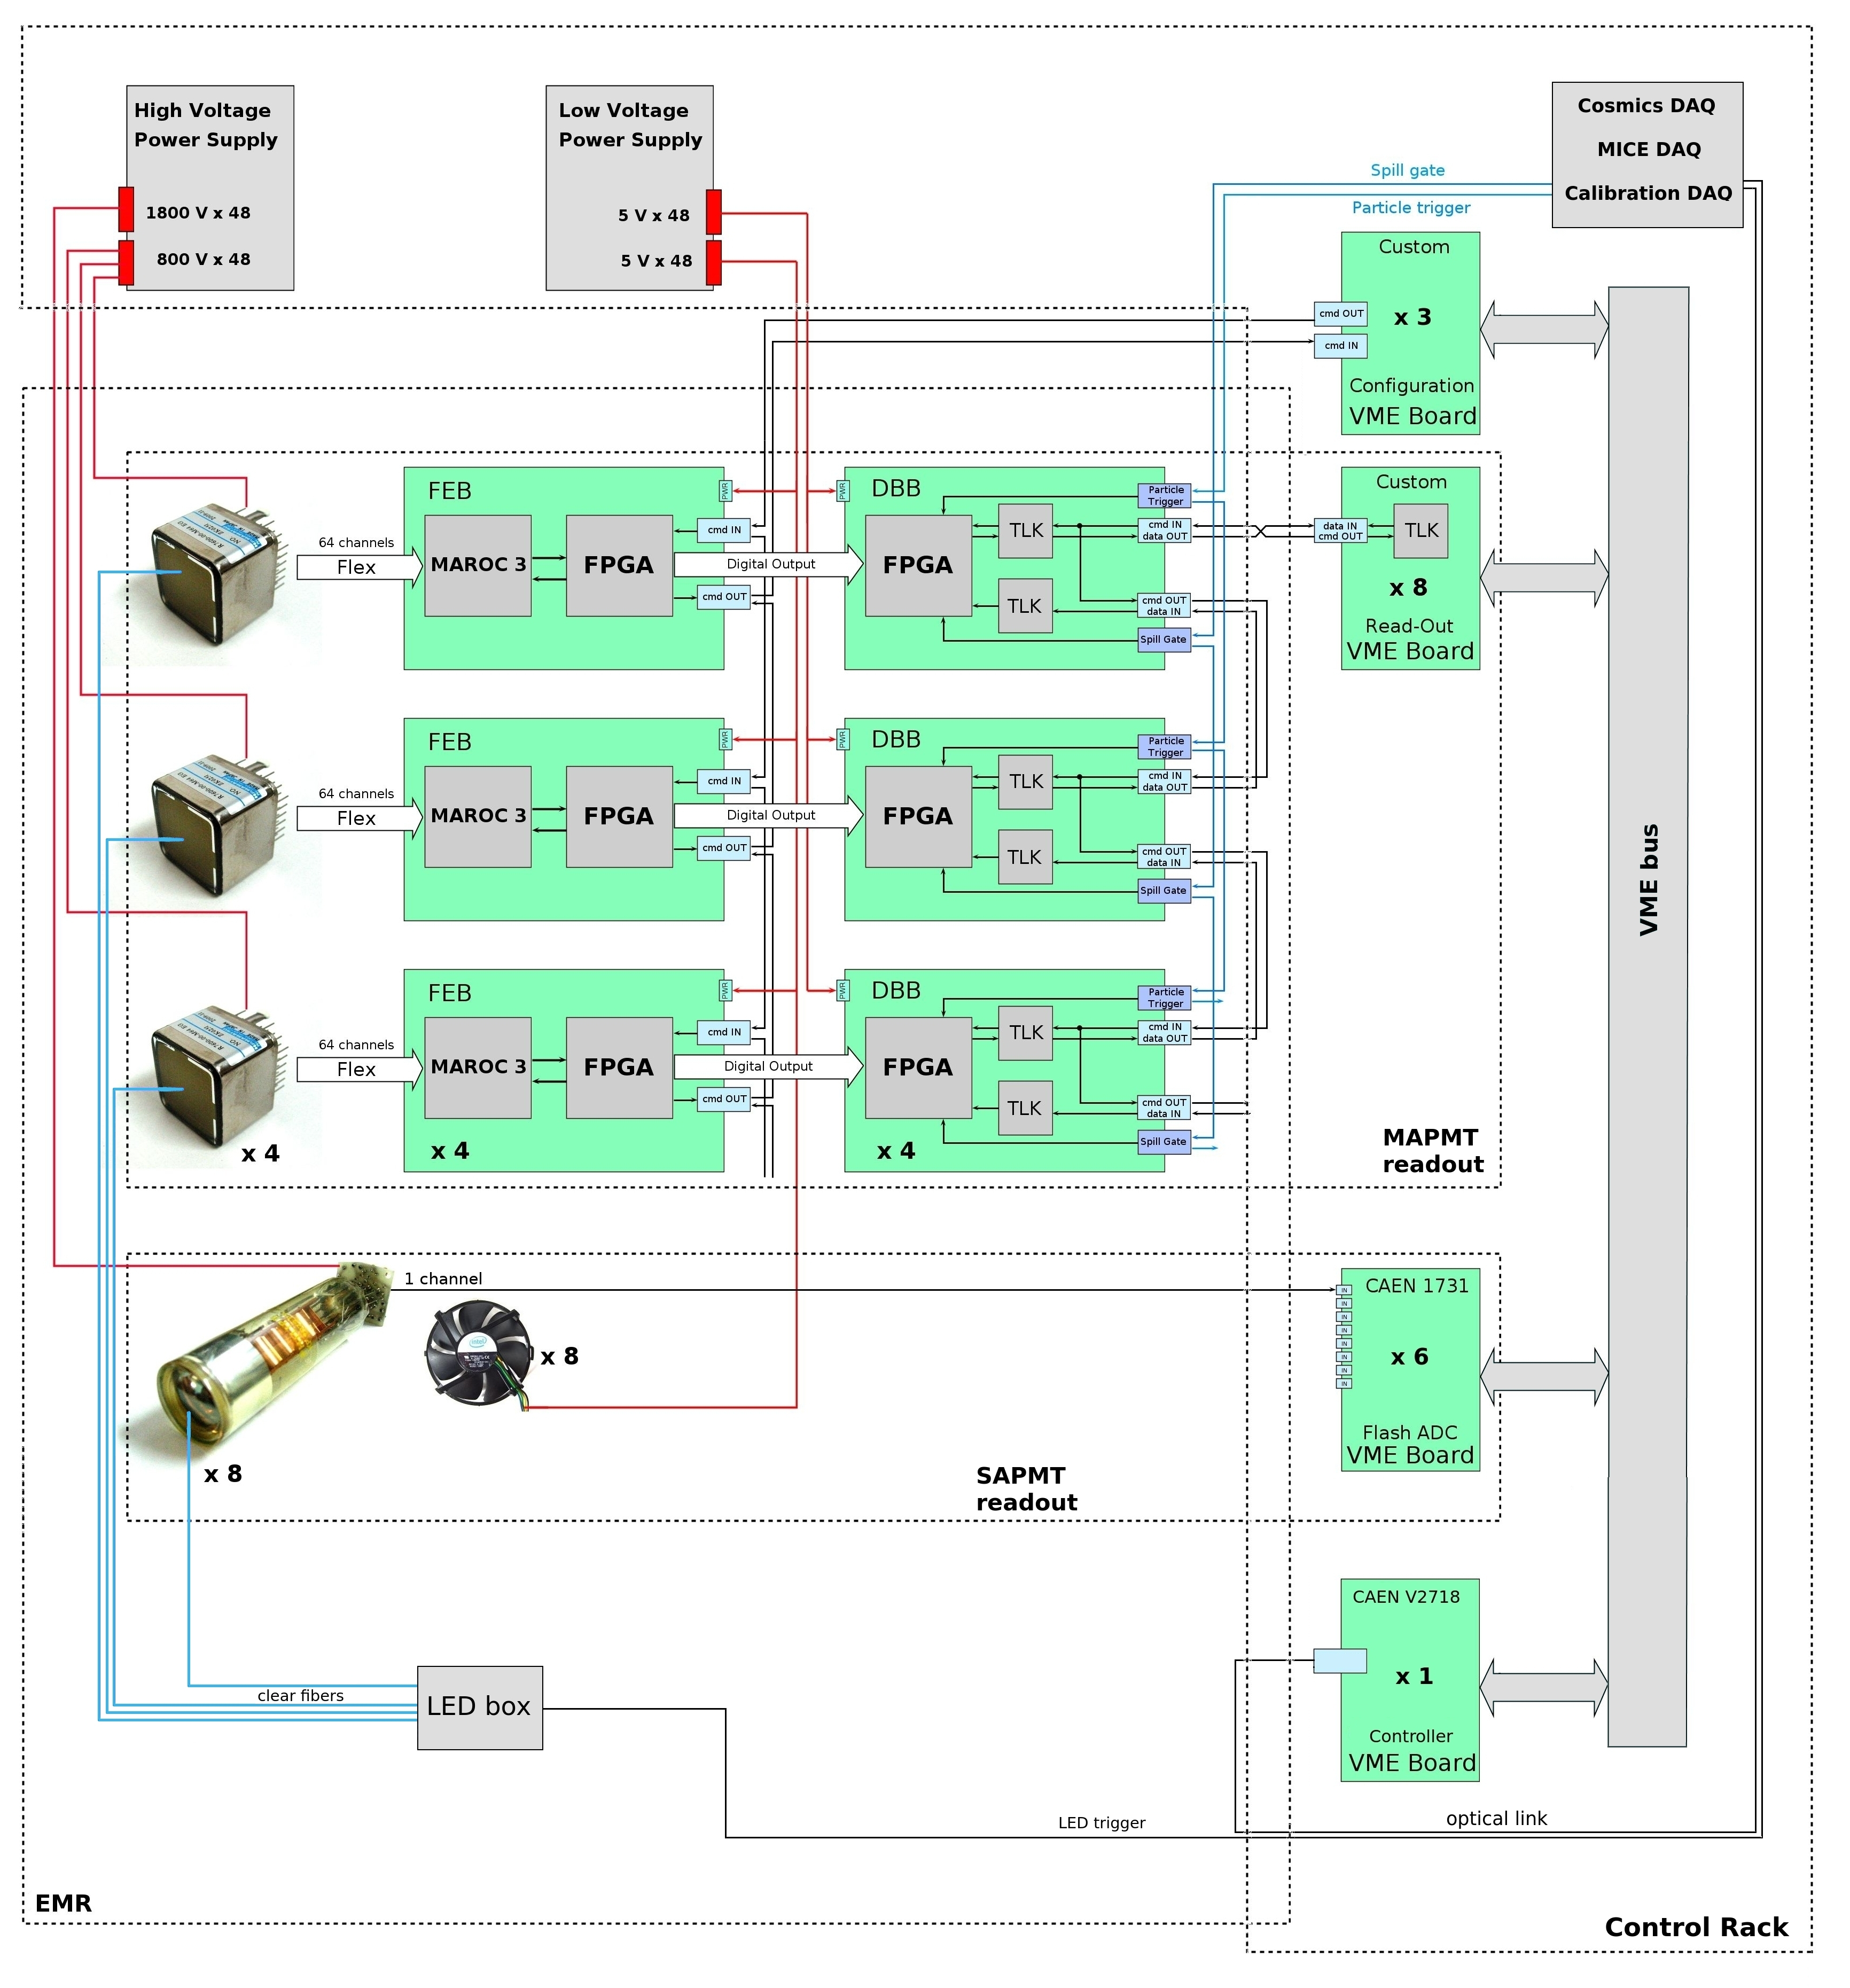
\includegraphics[width=\textwidth]{./EMR_electronics_layout}
 \caption[EMR electronics layout.]{EMR electronics layout. {\bf FEB:} front-end board for multi-anode PMT readout. {\bf DBB:} digitizer-buffer
 board. {\bf MAROC~3:} 64 channel readout ASIC for multi-anode PMT. {\bf MAPMT:} multi-anode PMT. {\bf SAPMT:} single-anode PMT.}
 \label{fig:EMR_electronics_layout}
\end{figure}

A schematic layout of the EMR electronics is shown in Figure~\ref{fig:EMR_electronics_layout}. The multi-anode PMT is connected via a flex cable
to a front-end board (FEB), which processes the signal and sends it to a piggy-back digitizer-buffer board (DBB) for digitization and storage.
The FEB is configured by the VME configuration board (VCB), which resides in the VME crate in the control rack. This board is able to configure
up to 16 FEBs, therefore three of them are required for the full detector. The DBBs are readout by groups of six. In each group the first DBB
is a master and the other five are slaves. All six boards are daisy-chained via ethernet cable and the master is connected to a VME readout board
(VRB), which transfers all the data from the six DBBs to the DAQ computer. In the whole detector there are 8 groups of DBBs, i.e. 8 VRBs are
installed in the control rack. 

\subsubsection{Front-End and Digitizer-Buffer Boards}
\begin{figure}[htp!]
 \centering
 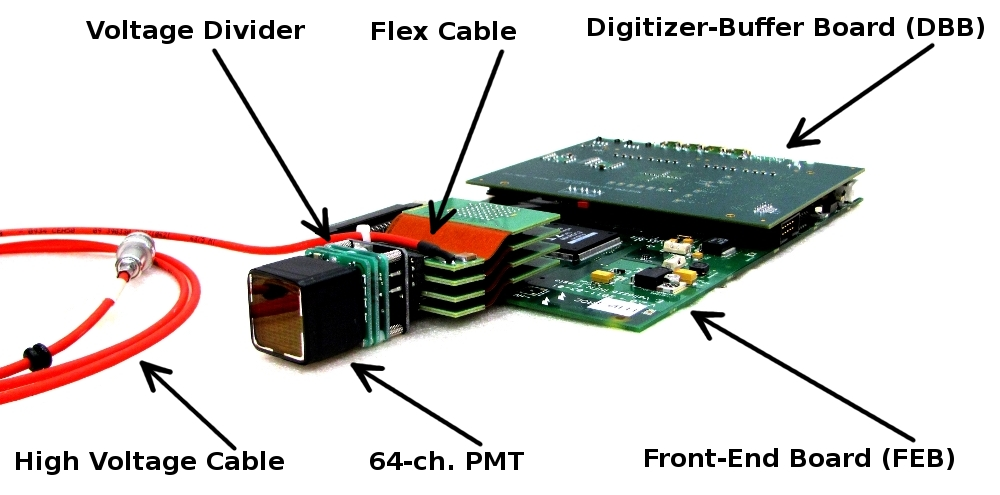
\includegraphics[width=0.8\textwidth]{./feb_dbb}
 \caption[Front-end and buffer board assembly]{Front-end and Digitizer-Buffer board assembly.}
 \label{fig:feb_dbb}
\end{figure}

The multi-anode PMT is readout by a dedicated front-end board equipped with piggy-back digitizer-buffer board \cite{Bolognini2011108}, which stores
hit information during a spill. Figure~\ref{fig:feb_dbb} show the full assembly that is mounted on every plane of the detector. It consists of a PMT
attached to a voltage divider, which is connected to a FEB through a flex cable. This cable also creates additional pressure between the PMT and
the fiber connector. The FEB is able to process all 64\footnote{Each EMR plane contains 59 scintillator bars which results in having 5 redundant
channels.} signals of the MAPMT thanks to a 64-channel ASIC\footnote{Application-Specific Integrated Circuit} called MAROC\footnote{Multi Anode
ReadOut Chip}\cite{maroc}.

The 64 analog signals are feed into the chip where they are processed in parallel: each channel consists of a pre-amplifier with a variable gain,
a tunable slow shaper and a sample and hold circuit for the analog readout, a tunable fast shaper and a discriminator for the digital one.
The MAROC ASIC provides 64 parallel digital outputs, which are forwarded to two high density connectors where a DBB is plugged. The width of the
discriminated signal represents a time over threshold measurement. One multiplexed analog output is also provided and this output is digitized by
an external ADC (AD9220, Analog Devices). It takes tens of microseconds (depending on the MAROC configuration used) to process all the multiplexed signals
and this dead time is not acceptable for the MICE DAQ duty cycle (a few hundred triggers per 1~ms spill). Therefore only time-over-threshold
measurement is used since it is practically dead-timeless.

The function of the FPGA chip\footnote{Altera Cyclone II (EP2C35F484C8N)} is mainly to forward data from the MAROC to the DBB and to send configuration
signals from the VCB to the MAROC and verify their status. The board has a separate power for analog and por the digital parts (both 5~V). The total
power consumption of the board is 0.6~Amp.

The two essential roles of the DBB are to sample 63 of the channels coming from the FEB plus an external trigger signal and to store the accumulated
digital data during the spill. It also has to transmit this data upon request of the acquisition system. The digitization starts when the board
receives the so called Spill Gate signal from an external LEMO connector. The number of clock ticks from the begging of the spill to the leading edge
and trailing edge of every discriminated signal coming from the FEB is recorded. The difference between the two measurements represents the time over
threshold of the original signal. The clock sampling rate is 400 MHz ($2.5 \ ns$ resolution). The external trigger signal is feed into one of the
64 input channel and is treated as any other signal. This signal does not serve as a trigger for the DBB itself, since the board records continuously
and all signals arriving within the spill gate are digitized and recorded. Nevertheless, the timing of the trigger signal is important, because it is
used to identify the records belonging to a given particle and for matching with the measurements recorded by the other detectors. The board also
calculates the width of every spill, counts the number of spills, number of triggers in the spills, and number of hits in every channel.

The architecture of the DBB is organized around a single FPGA\footnote{Altera Stratix II (EP2S30F484C3N)} that performs the sampling, data
buffering, and data-flow control functions of the board. Internal memory of the FPGA, configured as FIFO, is used to store the event data which is
a collection of leading and trailing edge timestamps that occurred on each channel during a specific spill. Two gigabit transceivers\footnote{TLK1501}
are interfaced to the FPGA to provide the physical transmission channels and form an upstream command link and a downstream data link. Six DBB's are
grouped together and daisy-chained with upstream and downstream links via ethernet cable. The first DBB in each group is directly connected to the
the VRB via four coaxial cables.

\subsubsection{VME Configuration Board}
The VCB is a single FPGA\footnote{Altera Cyclone II (EP2C50F484C8N} board designed to perform configuration of the MAROC chip on the FEB. The
communication between the two boards is realized via LVDS\footnote{Low-Voltage Differential Signaling, communication protocol.} signals driven and
received by LVDS drivers/receivers directly connected to a corresponding FPGAs. The MAROC chip is configured by TTL\footnote{Transistor-Transistor
Logic} signal composed of 830 bits which code the configuration parameters. The VCB can readout from the FEB the digitized measurement of the
MAROC analog output, but this is not implemented in the current design. The board communicates with the DAQ computer through the VME bus via the
VME controller. 

\subsubsection{VME Read-Out Board}\label{electronics:subsec:vme_readout_board}

One VRB performs the readout of a group of six DBBs. It is a single FPGA\footnote{Altera Cyclone II (EP2C50F484C8N)} board with a gigabit 
transceiver\footnote{TLK1501}, which drives the communication with the DBBs and four high-speed 16M-bit static RAMs\footnote{IS61WV102416BLL-10TLI
- SRAM, 16Mbit, 10ns, 48TSOP}, providing a local memory buffer. During the readout cycle, the transfer of the data between the DBBs and the DAQ computer
is executed in two steps. First, after a request from the DAQ computer, the VRB starts transferring data from the 6 DBBs. The gigabit transceiver is used
for this and the received data is temporarily stored locally. The four static RAMs, each organized as 16 bits data words, are grouped in two pairs,
providing the record of the DBB data, which is originally structured in 32 bits data words. Once the first part of the transfer is completed, and all
the data accumulated by the 6 DBBs during the spill is available in the local memory buffer of the VRB, the DAQ computer sends a second request which
triggers the transfer of this data over the VME bus.

Additional LVDS input/output connector is available at the front panel of the board. This connector does not have a specific function, and was used
mostly for debugging.

\subsubsection{Fast ADC Board}\label{electronics:subsec:fast_adc_board}

A waveform digitizer V1731, made by CAEN~\cite{V1731} is used to readout signals from single-anode PMTs. The digitizer has a sampling frequency of 500 M
samples per second (2~ns timing resolution). A pulse shape of each input signal is digitized by 8 bit ADC and continuously written in a circular memory
buffer. When a trigger\footnote{The same trigger signal, received by the DBBs} arrives the FPGA writes a certain number samples into the buffer, which
then is available for readout via the VME bus.

\subsection{Mechanics}\label{design:subsec:mechanics}

Total weight of the sensitive volume of the detector is almost 1 tonne. During construction and installation it is required to rotate and move the detector;
besides that it is meant to be transported in a truck over more then 1000 kilometres. Therefore a reinforced support frame (see Figure~\ref{fig:emr_support})
was design so that it can withhold the weight of the sensitive detector and all the stress that may happen during the transportation and installation. In its
final position the EMR is installed in such a way so that planes are located vertically perpendicular to a beam direction. 

\begin{figure}[htp!]
 \centering 
 \includegraphics[width=\textwidth]{./emr_support}
 \caption[EMR support frame]{EMR support frame. When installed in the MICE experimental hall, the EMR is integrated into the support structure of the other 
 downstream particle identification detectors.}
 \label{fig:emr_support}
\end{figure}

\begin{figure}[htp!]
 \centering
 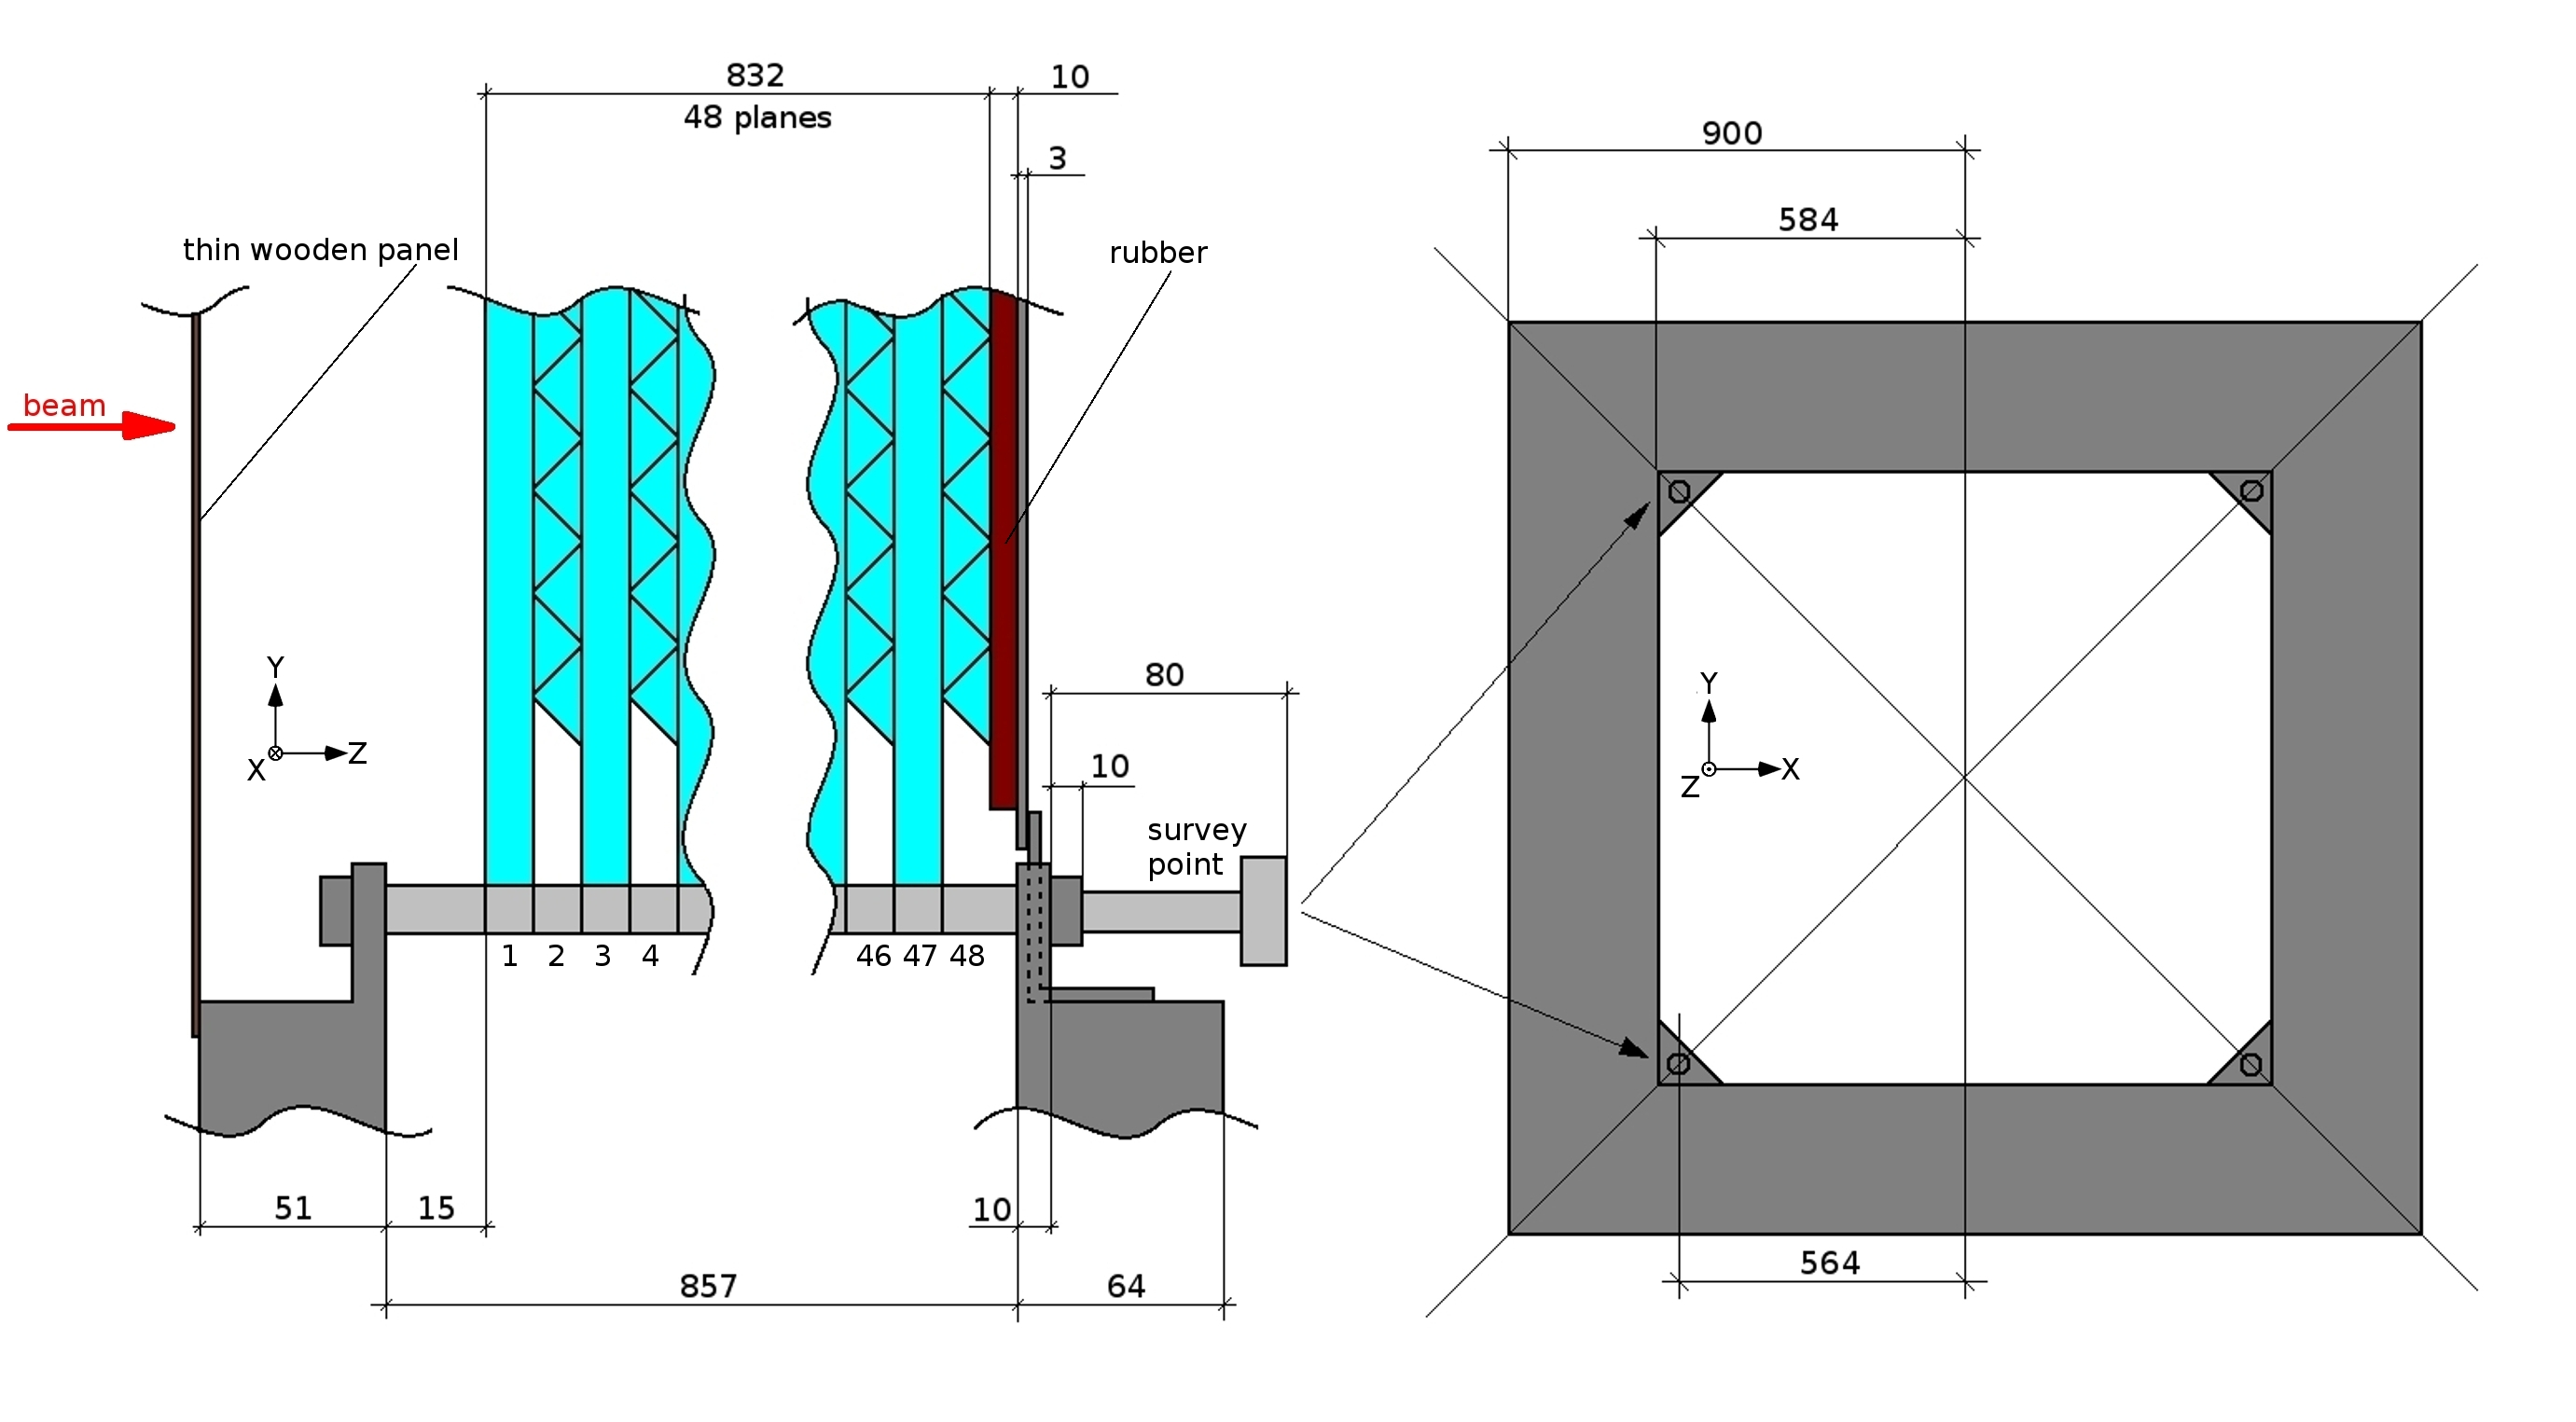
\includegraphics[width=0.9\textwidth]{./internal_dimensions}
 \caption[EMR dimensions]{EMR dimensions (mm).}
 \label{fig:internal_dimensions}
\end{figure}

Figure~\ref{fig:internal_dimensions} shows the location of the sensitive volume with respect to the support frame. The frame is covered with panels so that
the whole volume is light-tight. 5~cm thick iron plates are used to form a front panel magnetic shield (total weight 755~kg). The opening in the shielding
panel, which matches the size of the sensitive volume, is closed with a thin wooden end cap. The back panel is closed with a metal end cap (since it holds
the weight of the detector during assembly, when it is in horizontal position).

\section{Construction}\label{sec:construction}

All the construction work of the detector was done at University of Geneva. It is well known that exposure to ultra-violet (UV) light or high temperature
can damage the polystyrene molecules. This is especially important for fibers, because the damage decreases the light transmission. Therefore all activities
related to fibers and scintillators were performed in a UV clean room, i.e. lights and windows were covered with UV-protective films, with air conditioning
that kept the temperature around 25 \degree C. 

As it was already mentioned, the scintillator bars were produced at Fermilab. The first step in the construction was to glue the wavelength shifting fibers
into the bars. Transparent epoxy\footnote{Prochima E30 water effect resin ????} was used to glue the WLS fiber in order to increase the light collection
efficiency. Although 2832 bars were required for building the full detector, 3150 bars were glued and assembled with fiber connectors in
order to provide enough spares available. In the second step, both faces of the bar's fiber connectors were polished with a special polishing machine. Four
different grades of sand paper are used to achieve a mirror like quality of the polished surfaces. The last step is performed using a 1$\mu$m grade
diamond-based polishing paper.

Fiber bundles made of 60 clear fibers (see Figure~\ref{fig:fiber_bundles}) were manufactured. In the bundle, each fiber has an individual length, providing
a minimum bending radius, when connected. A fiber connector (see Figure~\ref{fig:fiber_connectors_cad}, bottom right) is glued at one end of each fiber. At
the other end all fibers are glued either in multi-anode or single-anode PMT connector (see Figure~\ref{fig:pmt_connectors}). Once glued, both fiber and PMT
connectors are polished on a bench, similar to the one used to polish all bar connectors. In total there were 96 fiber bundles (48 for each type of PMTs).

\begin{figure}[htp!]
 \centering
 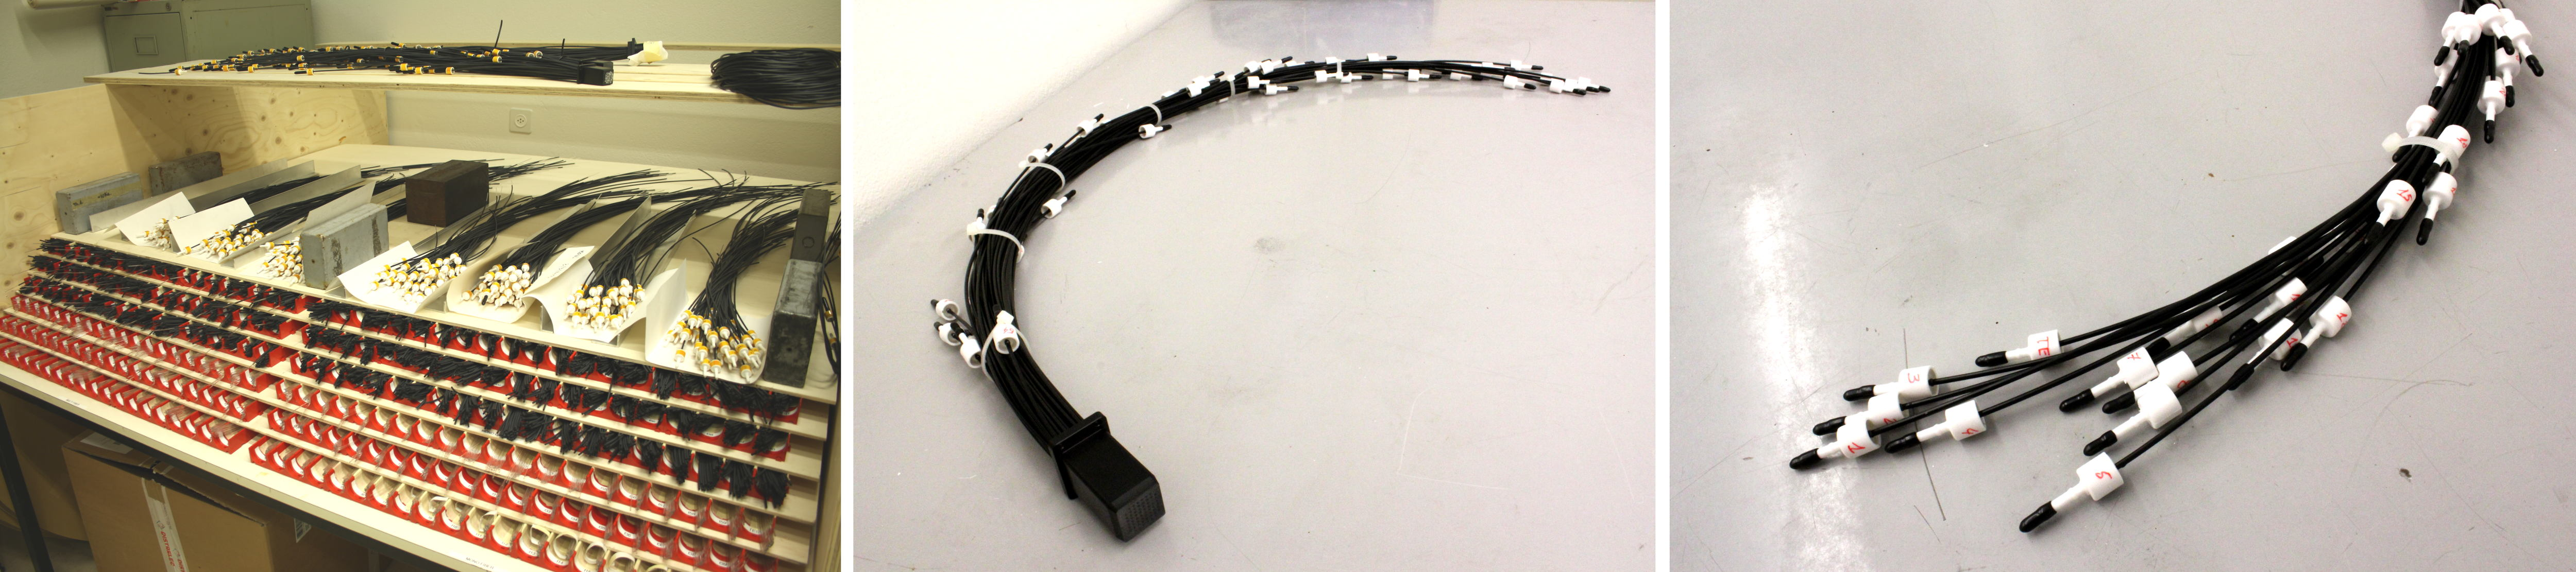
\includegraphics[width=\textwidth]{./fiber_bundles}
 \caption[Clear fiber bundles]{Clear fiber bundles. {\bf Left:} fiber pre-cut to the specified length. {\bf Centre:} PMT connector. {\bf Right:} fiber connector.}
 \label{fig:fiber_bundles}
\end{figure}

\subsection{Quality Tests}\label{construction:subsec:quality_tests}

Numerous quality test were implemented, in order to assure the best possible performance of the different components of the detector. 

A dedicated bar quality test bench was constructed in order to test the light transmission of each bar, including the transmission of the WLS fiber and the
quality of the two connectors. The test bench consisted of a LED\footnote{Light Emitting Diode} system, a holder for 4 scintillator bars and a digital camera,
all placed in a light-tight box. The LED system included blue LED, light mixing box and diffusers, providing that the light is homogeneous at the outputs,
where the bars under test are connected. The camera was taking a photo of the four connectors at the opposite side of the bars. Out of four bars one was a
reference and the measurements were normalized to it in order to take into account the effect of a possible LED instability and to have a possibility to
compare different measurements. An automated program was used to analyze the photos (Figure~\ref{fig:measurements} - left) and to calculate the light
intensity of each bar. Figure~\ref{fig:measurements} - right shows the distribution of the measured relative residuals of the light intensity. The relative
residual was defined as the difference between the measured value and the average value divided by the average. Only bars with a relative residual
intensity above -0.15 were accepted for plane assembly. Out of 3150 tested bars 305 bars (9.7\%) did not pass that requirement and were rejected.

\begin{figure}[htb]
 \centering
 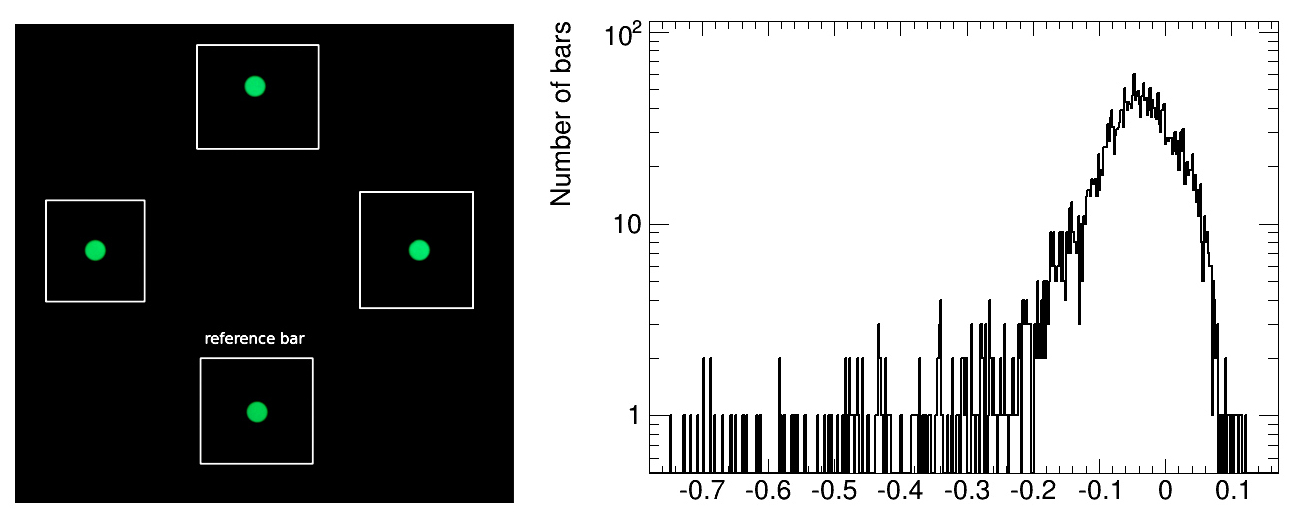
\includegraphics[width=.8\textwidth]{./measurements_cut}
 \caption[Bar quality test measurements]{Bar quality test measurements. {\bf Top left:} an example of one measurement, bottom bar is a reference. {\bf Top
 right:} distribution of the relative residual intensity.}
 \label{fig:measurements}
\end{figure}

A similar test was used to examine each EMR plane after the assembly. An LED tube attached to a single-anode PMT connector was used to send light through
the fibers (WLS and clear) all the way up to the multi-anode PMT connector, where a picture of the PMT mask was taken by a camera. Again,  an automated
program was used to analyse the photos (Figure~\ref{fig:plane_tests_one_planes} - left) and to calculate the relative residuals of the light intensity
of the individual channels (Figure~\ref{fig:plane_tests_one_planes} - right). This test verified the light transmission of the fiber bundles, but also
the quality of the interconnections between the WLS fibers and clear fibers. A plane was accepted only if the relative residual intensity of all 60
channels were above -0.4.

\begin{figure}[htb]
 \centering
 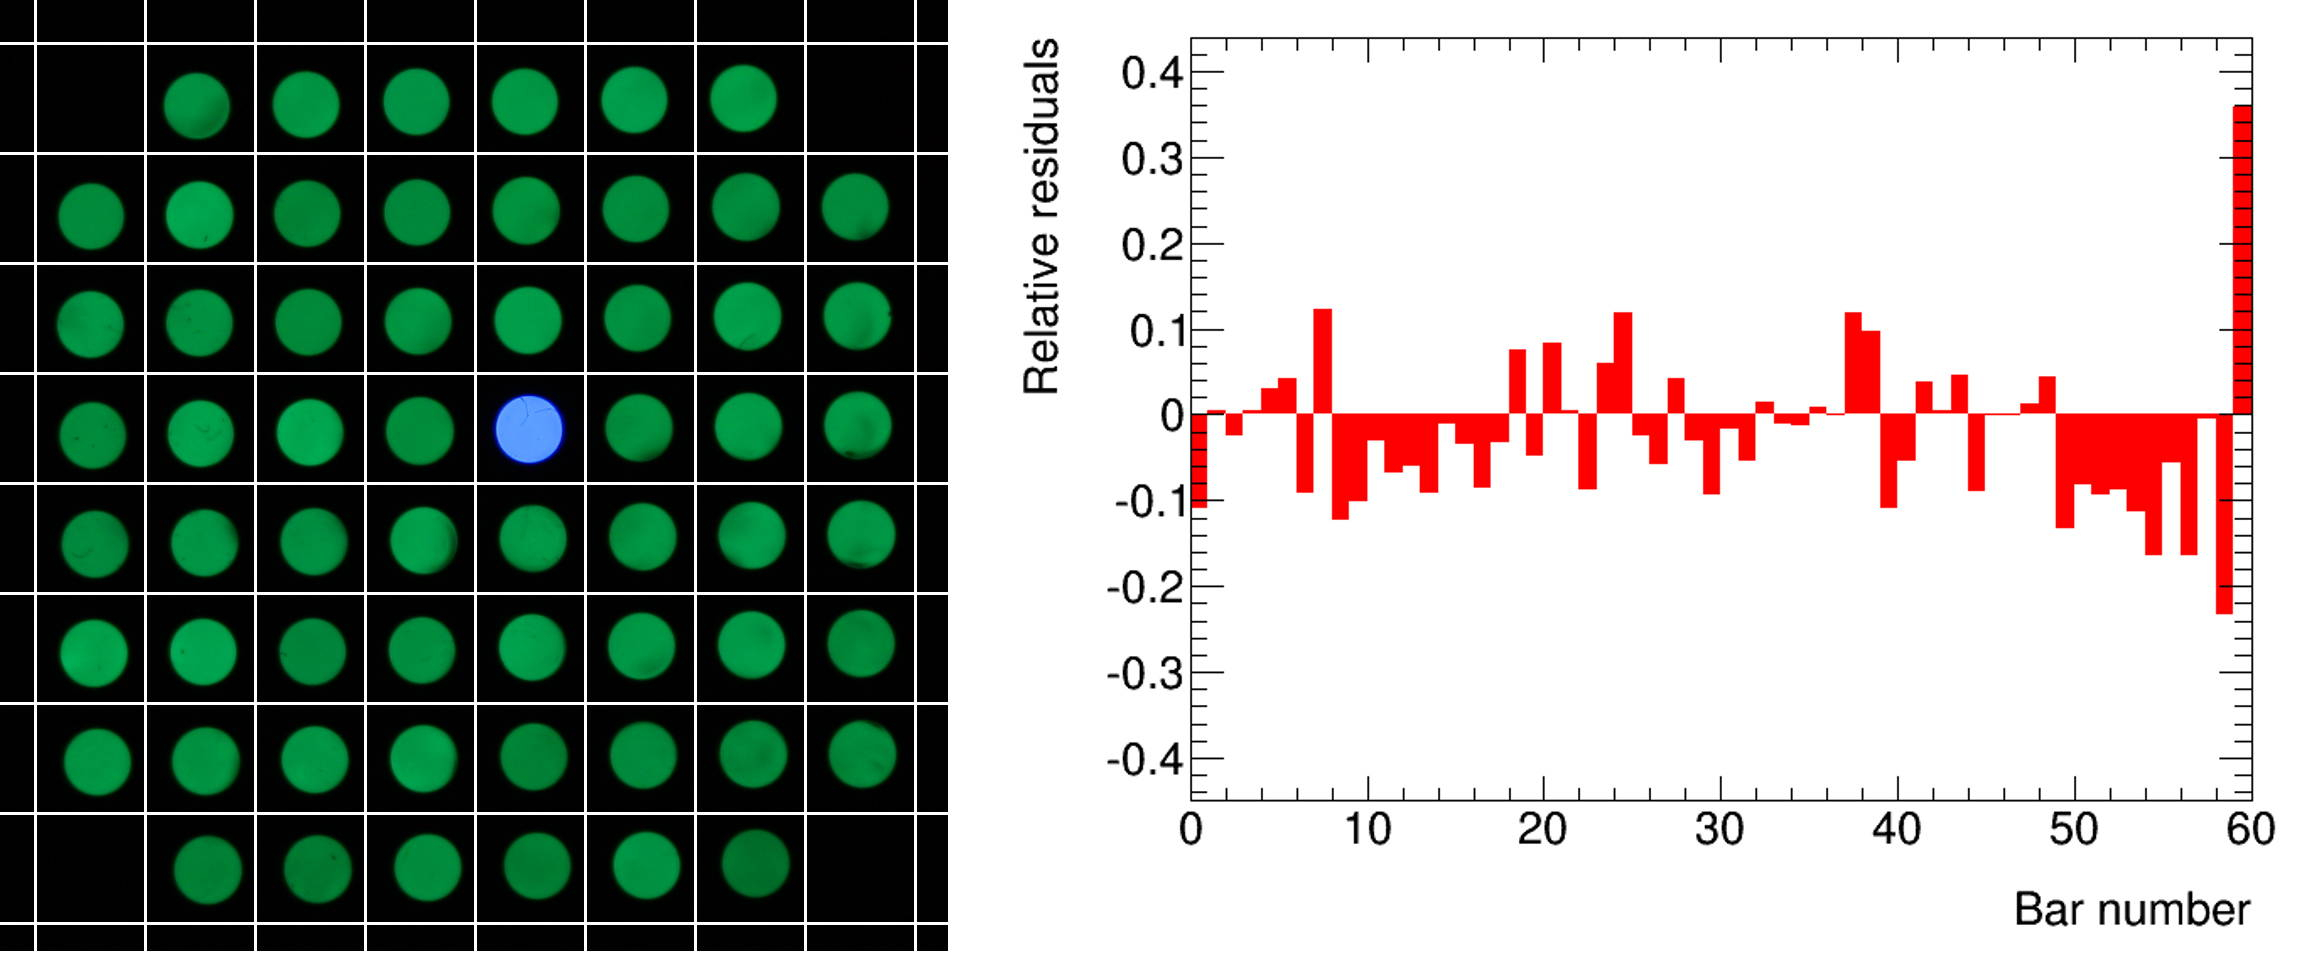
\includegraphics[width=0.8\textwidth]{./one_planes}
 \caption[Example of plane quality tests]{Example of plane quality test for one planes. {\bf Left:} PMT mask. {\bf Right:} relative residual intensity values
 for 60 channels, the last value is for a calibration channel.}
 \label{fig:plane_tests_one_planes}
\end{figure}


\begin{figure}[htb]
 \centering
 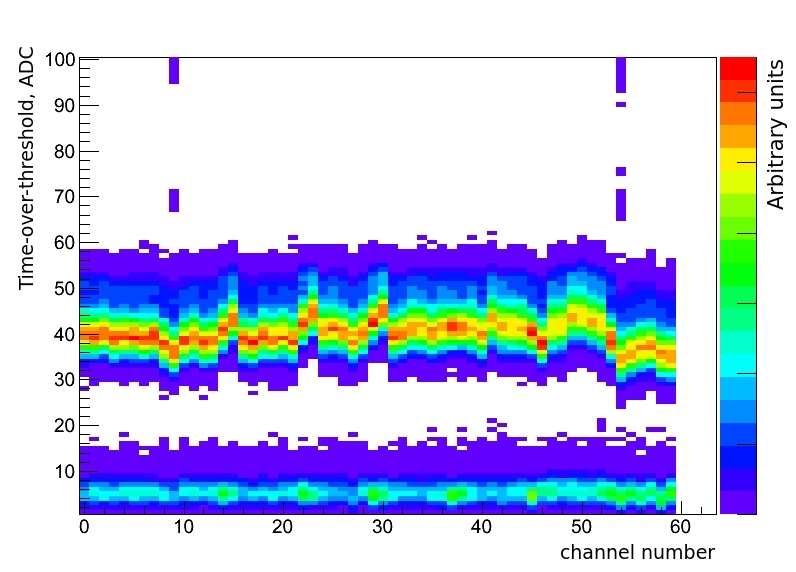
\includegraphics[width=0.45\textwidth]{./pl1_tot1}
 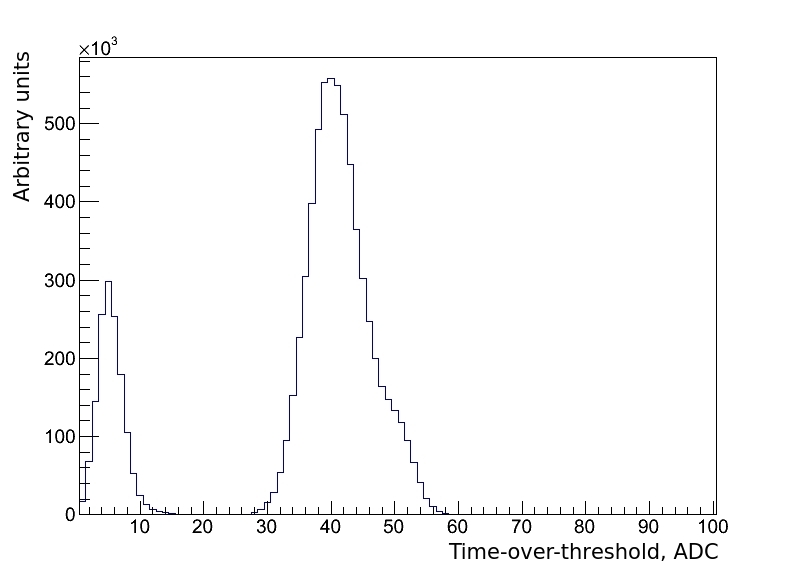
\includegraphics[width=0.45\textwidth]{./pl1_tot2}\\
 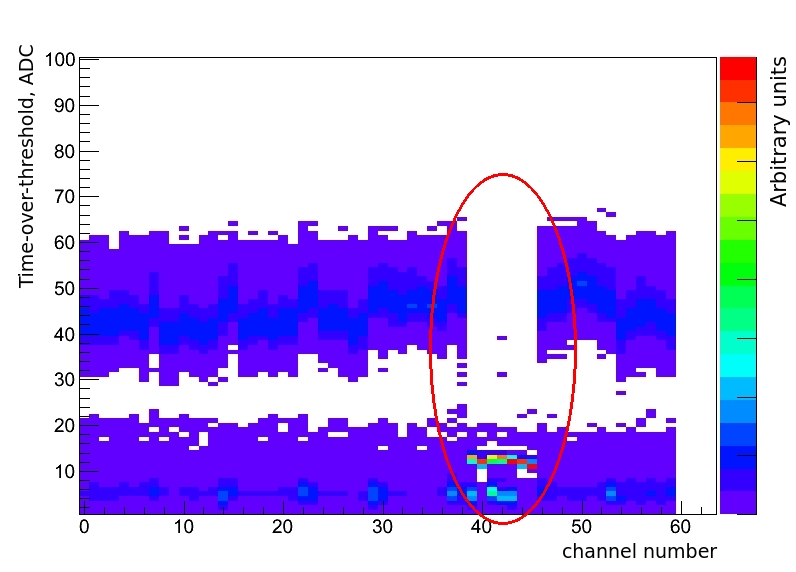
\includegraphics[width=0.45\textwidth]{./pl2_tot1}
 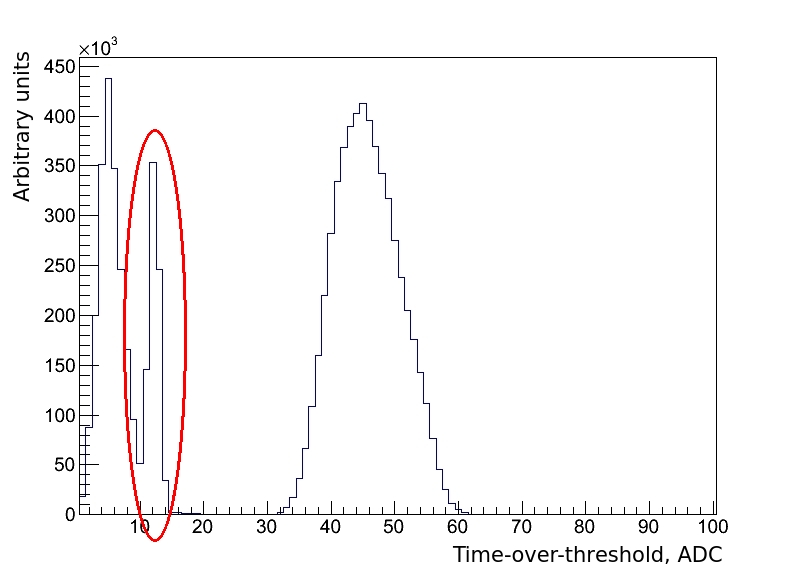
\includegraphics[width=0.45\textwidth]{./pl2_tot2}
 \caption[Electronics quality tests]{Electronics quality tests. {\bf Top:} functional board. {\bf Bottom:} faulty board. {\bf Left:} Time-over-threshold
 as a function of the channel number. Typical response to LED signal is around 40 ADC. Pedestal signal is around 5 ADC. Any faulty channel does not produce
 an adequate signal as seen in the bottom plot (channels 38 to 45). {\bf Right:} Distribution of the time-over-threshold for all channel in a given board.}
 \label{fig:tot_feb_dbb_test}
\end{figure}

A separate test bench was setup in order to verify the functionality of the three major components of the EMR electronics: the multi-anode PMTs, the 
front-end boards and the digitizer-buffer boars. It reproduced the full electronics chain used to readout the detector with the only difference that the
light is generated by a LED, power by a variable amplitude pulser. The LED was attached to the MAPMT injecting light in all channels at the same time. The
final measurement that is provided by the system is a time-over-threshold of the PMT signal. During the tests this measurement is used as a figure of merit
to characterize the electronics chain (PMT, FEB and DBB). Figure~\ref{fig:tot_feb_dbb_test} shows an example of a fully functional electronics chain (top)
and an example of a faulty electronics (bottom). Only boards, exhibiting a behaviour as in Figure~\ref{fig:tot_feb_dbb_test} - top, were accepted for
installation in the detector.

\subsection{Cosmic-based channel mismatch analysis}\label{sec:ch_mismatch}

The design of the EMR, involving the connection of external clear fibres to internal WLS fibres \cite{emr_design_change}, leaves room for human error in matching the two correctly.

An analysis was designed to verify the consistency of the cabling across the 2832 bars in the detector \cite{emr_xt, Francois}. The analysis uses the distance between each bar hit and its particle track as a tool to estimate the likelihood of mismatch. A mismatched channel is not reconstructed in the right location and is, on average, significantly less consistent with particle tracks.

Cosmic muons are particularly suited for this procedure as they traverse the whole detector without stopping and provide full coverage. At the time of data taking, the detector was positioned upright, planes perpendicular to the ground. Two pairs of planes (15--16 and 31--32) were used as particle triggers in coincidence with a software 3\,ms spill gate. Data was taken for 60 hours and yielded $\sim2.23\times10^5$ particle triggers.

Time-over-threshold measurements were recorded along with their timestamps in the 2832 channels for each trigger. Four dead channels were unveiled in plane 34. The amount of hits recorded in each bar is of order $\sim10^3$.

Two cuts are applied to the data sample in order to rid the muon tracks of artificial hits caused by crosstalk and noise. Crosstalk signals represent a small fraction of the total light yield and hence are rejected by placing a lower limit on the time-over-threshold. Restricting the delay between the trigger time and the hit time to a small interval gets rid of most of the noise.

To reconstruct tracks and calculate the distance of each hit from its particle trail, the hits are split into two projections $qz$, $q=x,y$. The plane ID of the channel hit provides the $z$ coordinate and the bar ID provides either $x$ for X planes or $y$ for Y planes. The $(q_i,z_i)$ coordinates are those of the barycentre of the triangular section or the bar corresponding to the hit. For a linear fit $q=a_qz+b_q$, the absolute distance between a hit $(q_i,z_i)$ and the track within a plane reads $\Delta q_i=|q_i-(a_qz_i+b_q)|$. For intuitiveness, distances are expressed in $\mathrm{b.u.}$ (bar units) in the following developments. A $\mathrm{b.u.}$ corresponds to the height of the triangular section or equivalently to the half width of its base.

The critical secondary variables that is measured for each channel are the ratios of mismatch, $R_i$. Given an integer $i$, the ratio $R_i$ corresponds to the fraction of the sample for which the bar is within $i\pm2/3$ $\mathrm{b.u.}$ off-track. For a distance distribution $f(\Delta y)$, the ratio is defined as

\begin{equation}
R_i=\frac{\int_{i-2/3}^{i+2/3}f(\Delta y)\mathrm{d}(\Delta y)}{\int_{0}^{2/3}f(\Delta y)\mathrm{d}\Delta y+\int_{i-2/3}^{i+2/3}f(\Delta y)\mathrm{d}\Delta y}.
\end{equation}

For instance, the ratio $R_1$ represents the probability of a bar of being mismatched by exactly 1\,$\mathrm{b.u.}$, i.e. to be swapped with an adjacent bar. It is shown in \cite{Francois} that $R_i$ is theoretically estimated to take values summarized in table~\ref{tab:mismatch_ratio} for different scenarios.

\begin{table}[!h]
 \centering
 \begin{tabular}{c|c|c|c|c}
  & \multicolumn{2}{c|}{Matched} & \multicolumn{2}{c}{Mismatched}  \\
  \hline
  & $xz$ proj. & $yz$ proj. & $xz$ proj. & $yz$ proj. \\
  \hline
  $R_1$ & 25.3\,\% & 32.2\,\% & 62.6\,\% & 66.1\%  \\
  $R_{i\geq2}$ & $\sim$0\,\% & $\sim$0\,\% & $\sim$100\,\% & $\sim$100\,\%
 \end{tabular}
 \caption{Mismatch ratios, $R_i$, for matched and mismatched bars in the two projections.}
 \label{tab:mismatch_ratio}
\end{table}

The mismatch ratio for adjacent bars was measured and is represented for each channel in fig. \ref{fig:ratio1}. The ratio distribution is represented next to it in log scale. The bulk of the distribution is centred around 28.88\,\%, consistent with the weighted average of the theoretical predictions for the two projections. Bars 47 and 48 of plane 44 record a ratio of 62.5$\pm$3.5\,\% and 57.2$\pm$3.2\,\%, respectively, significantly superior to the bulk and in agreement with the prediction. Their proximity to each other corroborates the hypothesis of a channel swap. The mismatch is fixed at the level of the channel map in the reconstruction.

\begin{figure}[htr!]
  \begin{minipage}[b]{.49\textwidth}
   \centering
   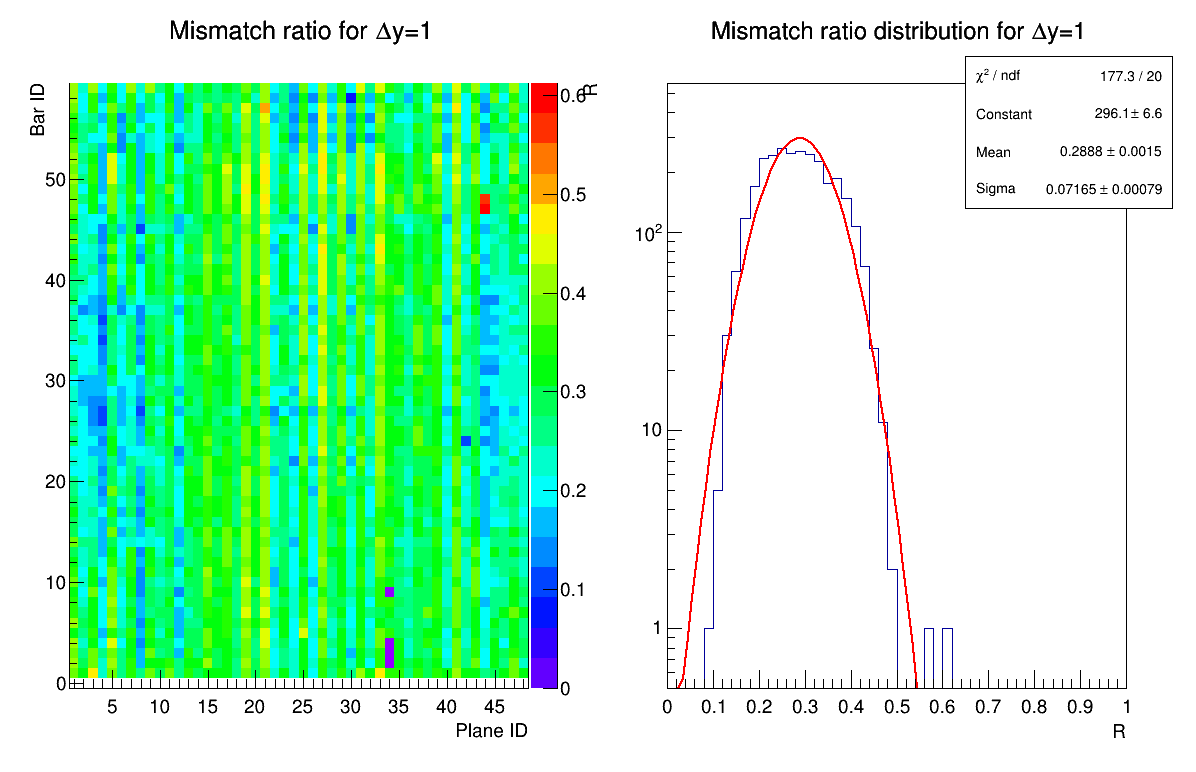
\includegraphics[width=\textwidth]{ratio1.png}
   \caption{Mismatch ratio for adjacent bars.}
   \label{fig:ratio1}
  \end{minipage}
  \begin{minipage}[b]{.49\textwidth}
   \centering
   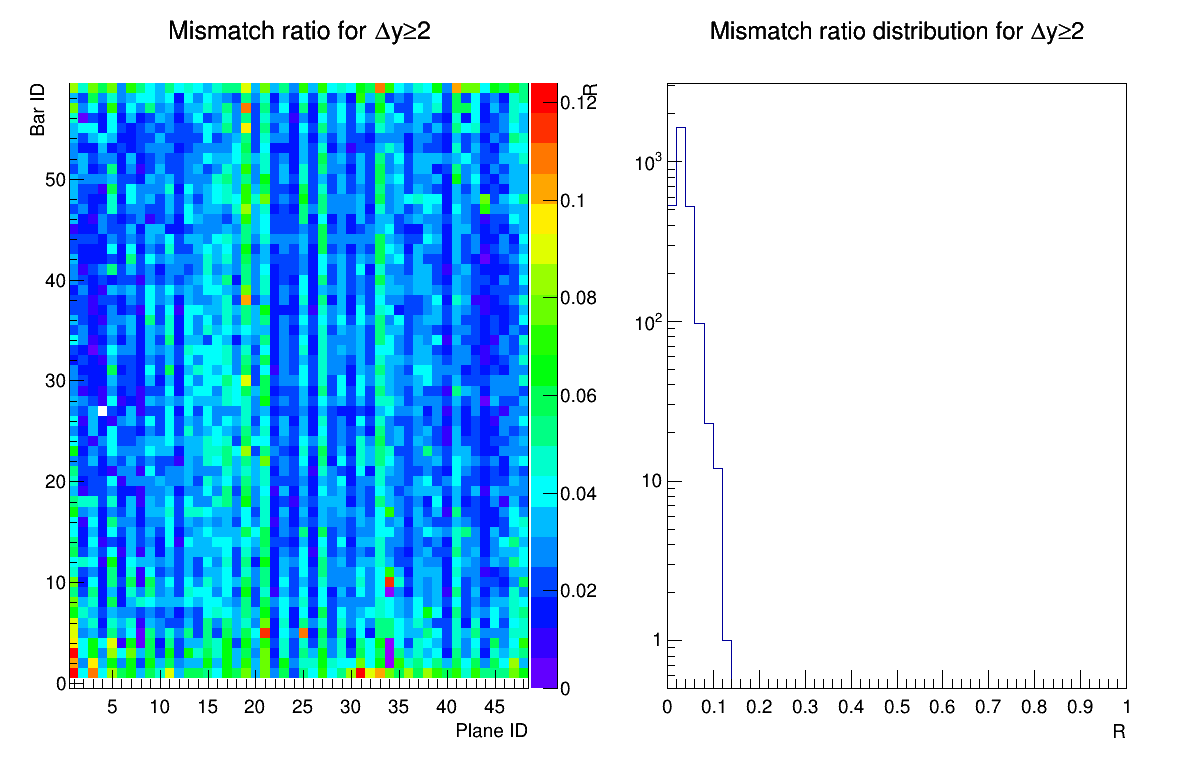
\includegraphics[width=\textwidth]{ratio2.png}
   \caption{Mismatch ratio for distant bars.}
   \label{fig:ratio2}
  \end{minipage}
\end{figure}

The same analysis has been conducted for potential mismatches of two bars or more, $R_{i\geq2}$. Figure~\ref{fig:ratio2} represents the value of that ratio for each channel. The results strongly reject any mismatch at this level.

\subsection{LED-based crosstalk analysis}\label{sec_xt}
The EMR is susceptible to two types of crosstalk: optical crosstalk, i.e. a single fibre of a bundle shining on more than one channel of the multi-anode photomultiplier (MAPMT) mask, and anode crosstalk, i.e. a photo-electron leaking from a dynode to an adjacent accelerating structure. An analysis was developed in \cite{emr_xt, Francois} to evaluate the significance of this phenomenon.

Cosmic or beam data are poorly suited for this analysis. A real particle often hits two bars or more within the same plane which makes it impossible to disentangle real signals from crosstalk in neighbouring channels. An LED light source is a more reliable tool to drive the analysis. Light is transported from an LED driver through 48 clear fibres to one specific channel of each MAPMT. It has four directly adjacent channels: top (N), bottom (S), left (W) and right(E). This method ensures that hits in the adjacent channels are caused by crosstalk only.

The LED driver was tuned with a variety of voltages ranging from 11.0 V to 22.0 V by steps of 0.5V. The trigger consisted in the coincidence of an arbitrary spill gate and hits in a channel 0. For each setting, 10000 pulses were recorded. The mean time-over-threshold in the test channel is represented as a function of the LED driver voltage in figure~\ref{fig:voltage}. The green area represents the voltage region for which the recorded time-over-threshold are consistent with cosmic muons figures.

\begin{figure}[htr!]
  \begin{minipage}[b]{.49\textwidth}
   \centering
   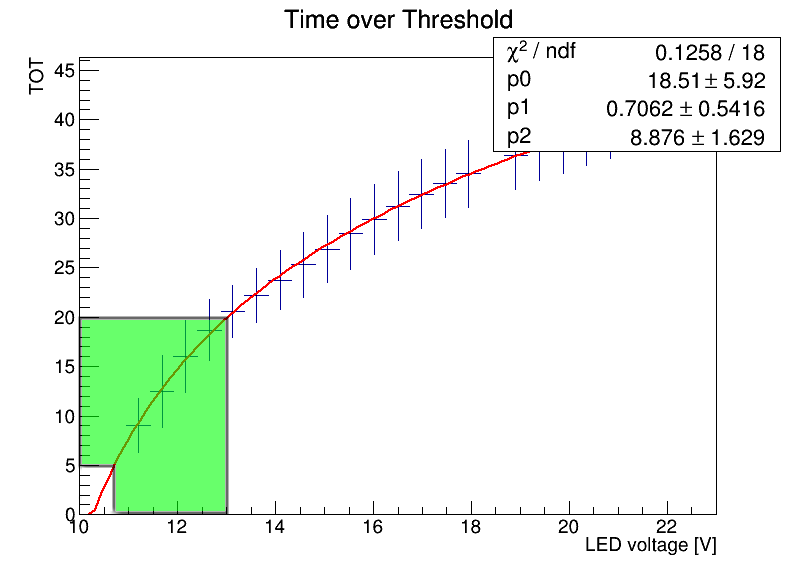
\includegraphics[width=\textwidth]{settings.png}
   \caption{Mean time-over-threshold in the test channel as a function of the LED driver voltage.}
   \label{fig:voltage}
  \end{minipage}
  \begin{minipage}[b]{.49\textwidth}
   \centering
   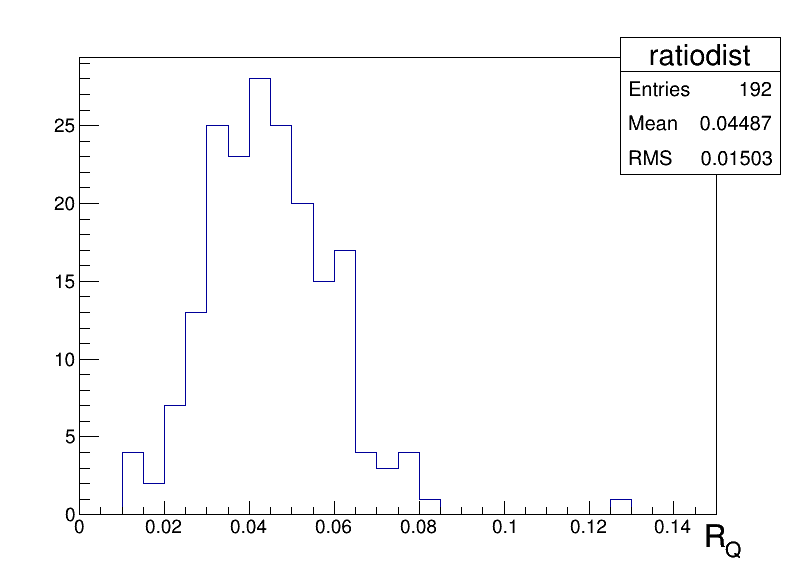
\includegraphics[width=\textwidth]{ratiodist.png}
   \caption{Fraction of the original charge that can leak in adjacent channels.}
   \label{fig:ratio_dist}
  \end{minipage}
\end{figure}


The first parameter that characterizes the crosstalk is the charge ratio, $R_Q^i$, between the signal amplitude in an adjacent channel $i$ and the primary amplitude in the test channel. The charge is not measured directly but is related to the time-over-threshold through $Q=e^{a\times \mathrm{ToT}+b}$. The parameters of the exponential are fitted for each plane to the relation between the single-anode photomultiplier charge and the time-over-threshold in the test channel. The ratio subsequently reads
\begin{equation}
R_Q^i=\frac{Q_i}{Q_0}=\frac{e^{a\times ToT_i+b}}{e^{a\times ToT_0+b}}=e^{a(ToT_i-ToT_0)}.
\end{equation}

The ratio is measured for the highest achievable LED voltage setting as the resolution evolves as $1/\sqrt{Q}$. The ratio measured in the 192 readout channels (directly adjacent N,S,W,E channels of each plane) is represented in figure~\ref{fig:ratio_dist}. The fraction of the original signal that typically leaks in adjacent channels is $4.49\pm0.11\,\%$.

The second parameter used to characterize the crosstalk is the rate. The measured quantity is the ratio $R_N^i$ of hits in a surrounding channel $i$ to the total amount of pulses generated in the test channel. This quantity is measured in the 192 readout channels for a voltage setting in the green area of figure~\ref{fig:voltage}, corresponding to MIP-like signals, and represented in figure~\ref{fig:rate_dist}. The average rate fraction is $0.20\pm0.01\,\%$, well within design requirements.

\begin{figure}[htr!]
  \begin{minipage}[b]{.49\textwidth}
   \centering
   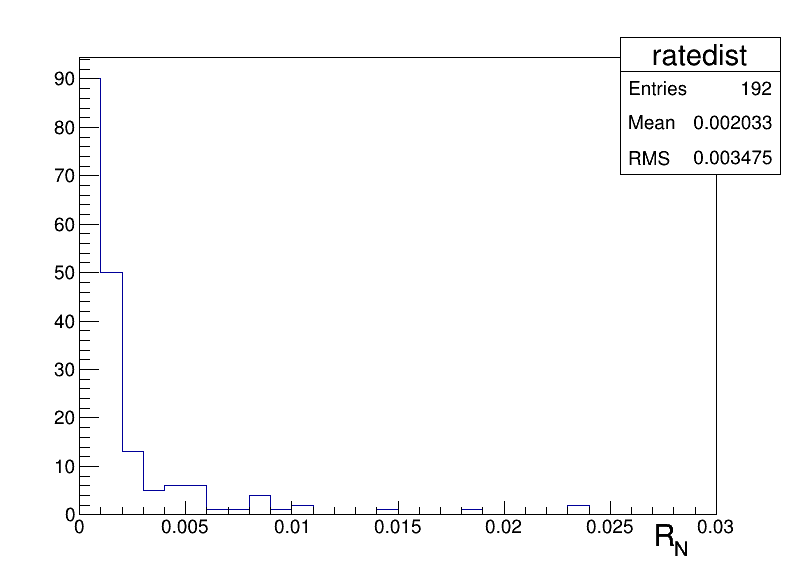
\includegraphics[width=\textwidth]{ratedist.png}
   \caption{Fraction of the time a signal produces crosstalk for a typical MIP energy loss.}
   \label{fig:rate_dist}
  \end{minipage}
  \begin{minipage}[b]{.49\textwidth}
   \centering
   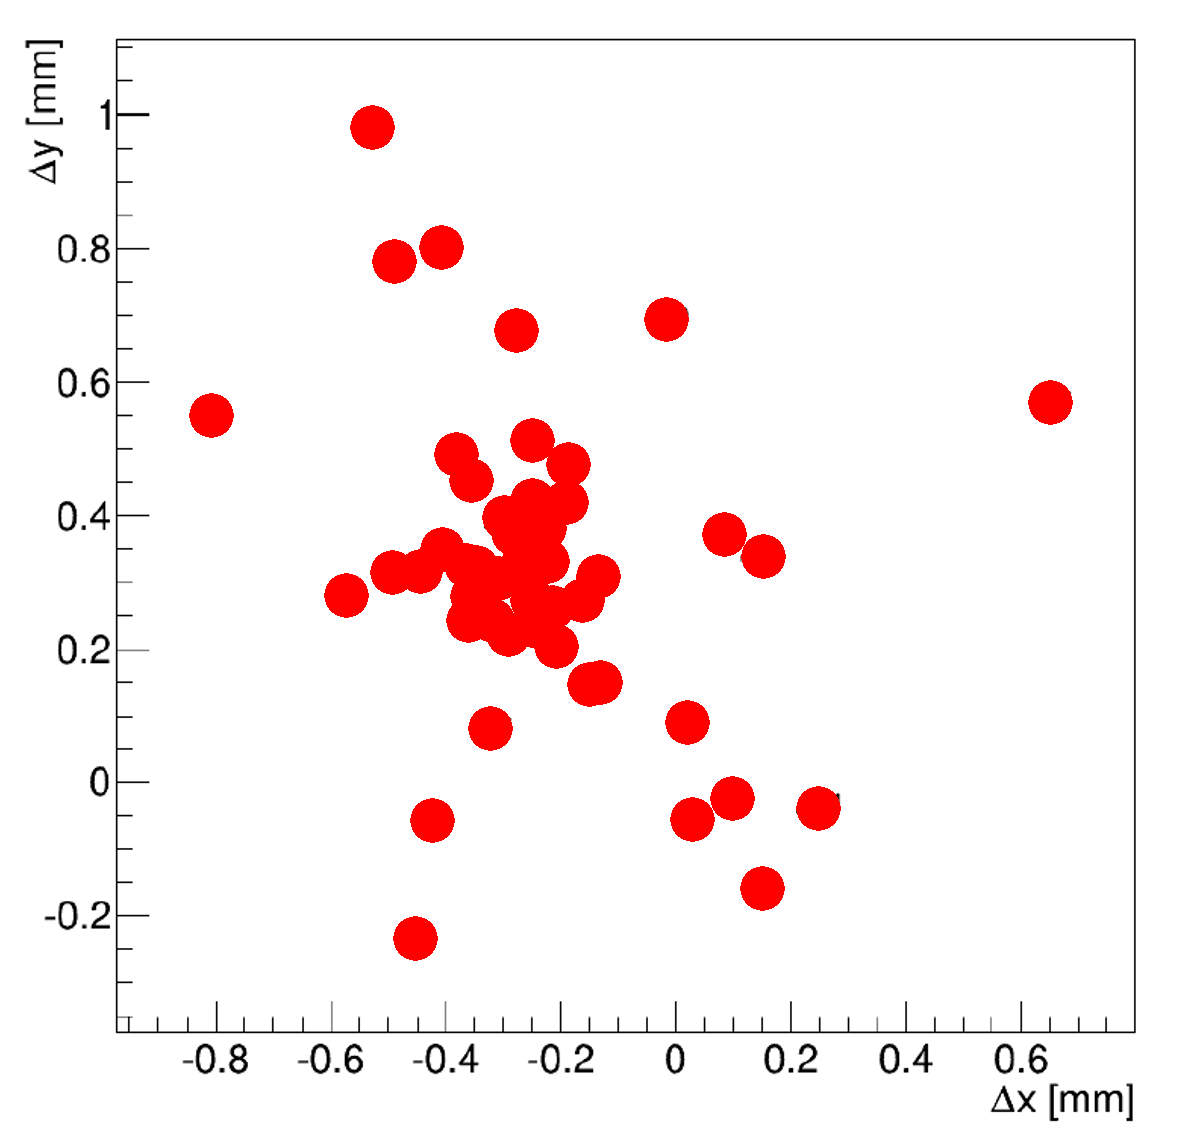
\includegraphics[width=.7\textwidth]{misalignment.jpg}
   \caption{Misalignment of the MAPMT mask with respect to the fibre bundle for the 48 planes.}
   \label{fig:misalignment}
  \end{minipage}
\end{figure}

The measurement of the crosstalk rate in the adjacent channels also provides a measurement of misalignment of the MAPMT mask with respect to the fibre bundle. If a mask is shifted, light is more likely to leak and create signals is the channel towards which it is offset. The centre of the mask with respect to the centre of fibre bundle is computed through

\begin{equation}
(x_C,y_C)=\left(\frac{\sum_ix_iw_i}{\sum_iw_i},\frac{\sum_iy_iw_i}{\sum_iw_i}\right),
\end{equation}

with ($x_i,y_i$) the coordinates of the surrounding channels and $w_i$ the amount of hits recorded in them. The resolution is function of $1/\sqrt{N}$, $N$ the amount of signals recorded, hence a high voltage is chosen for this analysis. The results for the 48 planes are presented in figure~\ref{fig:misalignment}. There is a noticeable cluster around $(-0.3,0.3)$ but nothing that could impair the detector.



\section{Transportation and installation at Rutherford Lab}

The total weight of the EMR detector is 2.5 tonnes. Therefore a special care was taken to insure safety and shock-free transportation of the detector.
Namely, the detector was attached to special shock absorbers designed to withstand this weight and allow for shock absorption in all three directions. The
shock absorbers were then attached to a pallet by which the detector was handled. It was placed in a truck and transported from University of Geneva to
Rutherford Lab (Didcot, Oxfordshire, UK) over more than 1100 kilometres. 

Once delivered to the Rutherford Lab the EMR detector was installed in the MICE hall and positioned vertically at the end of existing MICE beamline. Later,
it was exposed to a beam which parameters were varied in order to achieve different beam compositions and momenta. This data was used to verify the designed
functionality of the detector, i.e. the ability to distinguish different particle types (muons, electrons and pions) and to measure their ranges
\cite{performance}. 

\section*{Acknowledgement}
The work described here was made possible by grants from Swiss National Science Foundation, in the framework of the SCOPES programme and the European Community
under the European Commission Framework Programme 7 (AIDA project, grant agreement no. 262025. We gratefully acknowledge all sources of support.


\bibliographystyle{unsrt}
\bibliography{bibliography}

\end{document}
